
% A LaTeX (non-official) template

\documentclass[a4paper,12pt]{article}
\usepackage[utf8]{inputenc}
\usepackage[T1]{fontenc}
\usepackage[spanish]{babel}
\usepackage{graphicx}
\graphicspath{{images/}}
\usepackage{amssymb,amsmath,bbm}
\usepackage{caption}
\usepackage{subcaption}
\usepackage[]{units}
\usepackage{array}
\usepackage{bm}
\usepackage{float}
\usepackage{tabularx}
\newcolumntype{L}[1]{>{\raggedright\arraybackslash}p{#1}}
\newcolumntype{C}[1]{>{\centering\arraybackslash}p{#1}}
\newcolumntype{R}[1]{>{\raggedleft\arraybackslash}p{#1}}
\usepackage{siunitx}
% \usepackage{color}
\usepackage[dvipsnames]{xcolor}
\usepackage{multirow}
\usepackage{layouts}
\usepackage{enumitem}
\usepackage{geometry}
\usepackage{verbatim}
\usepackage{steinmetz}
\usepackage{hyperref}
\usepackage[ampersand]{easylist}
\usepackage{gensymb}
\usepackage{appendix}
\usepackage{listings}
\usepackage{multicol}
\usepackage{xcolor}
\usepackage{makecell}
\usepackage[nottoc,numbib]{tocbibind}
\usepackage{url}
\hypersetup{
    colorlinks,
    linkcolor={red!50!black},
    citecolor={blue!50!black},
    urlcolor={blue!80!black}
}
\parskip=5pt


\lstdefinestyle{lststyle}{
  breaklines=true            
}

\lstset{style=lststyle}

\title{
	\normalfont \huge 
	\textsc{UNIVERSIDAD DE BUENOS AIRES \\
		Facultad de Ingeniería} \\
	\begin{center}
		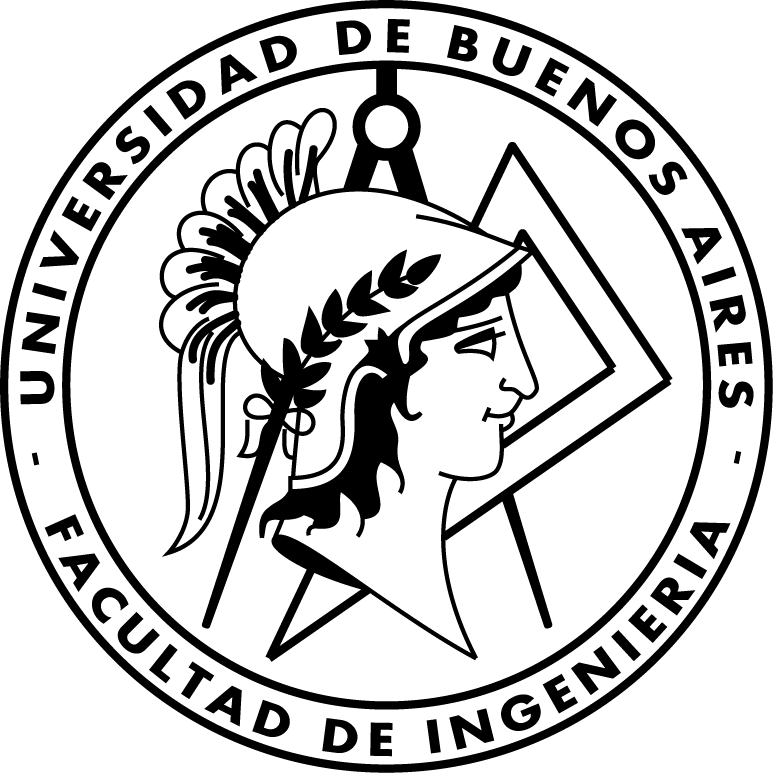
\includegraphics[width=0.5\textwidth]{images/Logo-fiuba_big.png}
	\end{center}
	\large \textbf{Tesis} \\
	\textsc{\large Estudio de sistemas de filtrados de ruidos no estacionarios presentes en señales de habla.}
}

\begin{document}

\pagenumbering{gobble}

\maketitle
~
\begin{center}
     \centering
     Espósito, Diego -\ desposito@fi.uba.ar - \ $\#95669$\\
\end{center}

\rule{\linewidth}{0.3pt} \\[3pt]

\newpage

\section*{\hfil Resumen \hfil}

\noindent El filtrado de ruidos no-estacionarios presentes en señales de habla es un problema que en los últimos años atrajo gran atención debido al proceso de digitalización acelerada que está sufriendo muchas de las actividades que el ser humano hace diariamente. Antes del gran desarrollo que tuvieron las redes neuronales profundas, el marco general para el filtrado de ruido no-estacionarios era por medio de la utilización de filtros adaptativos. El objetivo de esta tesis será comparar el filtrado de ruidos no-estacionarios por medio de filtros adaptativos y por medio de filtros neuronales, utilizando métricas objetivas como la medida de calidad PESQ y la medida de inteligibilidad STOI. Los resultados encontrados en este trabajo, sugieren que en condiciones de bajo nivel de ruido, un filtro neuronal es capaz de igualar el desempeño de un filtro adaptativo o incluso mejorarlo.

\newpage

\section*{\hfil Agradecimientos \hfil}

\noindent La culminación de una tesis de grado no es solo fruto del esfuerzo dedicado para realizarla sino que de todo el trabajo realizado a lo largo de todos los años que conlleva estudiar una carrera de grado. Es por esto que no solo le quiero agradecer a aquellos que me acompañaron durante la elaboración de esta tesis sino que a todas aquellas personas que estuvieron conmigo a lo largo de este tiempo.

\noindent En primer lugar le quiero expresar mi eterno agradecimiento a mi esposa, quien me acompañó desde el inicio de esta etapa. Por su infinita paciencia durante los largos periodos de estudio. Por su incondicional apoyo durante toda la carrera. Por enseñarme a tener una mirada menos analítica y estructura y por enseñarme a tener mayor capacidad reflexiva.

\noindent En segundo lugar, le quiero agradecer a mi familia. A mi hermano por su eterno optimismo y por inspirarme a siempre ser mejor e ir un poco mas lejos. A mis padres por enseñarme todo lo que soy, por darme la educación que me dieron y por acompañarme y apoyarme en todos mis proyectos. También le quiero agradecer a mis abuelos y abuelas, a mis tíos y a mis primos por siempre estar conmigo.

\noindent Le quiero agradecer a mis amigos que en todos aquellos momentos donde por tener que estudiar no pude estar, me apoyaron y me motivaron a seguir adelante.

\noindent A mi tutor el Dr. Ing. Juan Ignacio Giribet por su acompañamiento.

\noindent A los jurados la Dr. Ing. Patricia Pelle, el Dr. Ing. Claudio Estienne y al Ing. Ricardo Veiga por usar su tiempo para evaluar esta tésis.

\noindent Por último le quiero agradecer a todos aquellos profesores y educadores que formaron parte de mi educación por haber aportado ese granito de arena que me hace ser el profesional que hoy en día soy.

\newpage

\tableofcontents

\newpage

\pagenumbering{arabic}

\section{Introducción}

\subsection{Descripción}

El presente trabajo analiza e investiga las limitaciones y bondades de dos tipos de filtros de ruidos no estacionarios, presentes en señales de habla.

Se busca comparar una técnica tradicional de filtrado, como es la de los filtros adaptativos con un filtro basado en redes neuronales profundas (DNN por sus siglas en ingles). Se los evaluará utilizando una variedad de ruidos no estacionarios presentes en aplicaciones del mundo real con el fin de investigar el comportamiento de cada uno de ellos.

\subsection{Antecedentes}

Usualmente las aplicaciones que trabajan con señales de habla captadas por uno o más micrófonos, como puede ser una aplicación de videoconferencias, poseen distintos tipos de filtros que permiten reducir el ruido presente en la señal de habla y así transmitir una señal de habla más clara. Distintas técnica son usualmente utilizadas para lograr dicho objetivo como puede ser la llamada sustracción espectral \cite{espectral_subtraction} o un filtro de Wiener \cite{philipos_book_speech_enhancement}.

Este tipo de filtros logran su objetivo para ruidos que son del tipo estacionario como por ejemplo, el ruido generado por el sistema de refrigeración de una computadora. Sin embargo fallan cuando la señal de habla se encuentra en un ambiente con ruidos del tipo no-estacionarios como por ejemplo, el ruido generado por escribir en un teclado, una impresora funcionando, el ladrido de un perro, tráfico, etc.  

En lo que concierne al filtrado de ruidos no-estacionarios, algunos trabajos abordaron el problema con técnicas de modelado estadístico como en \cite{speech_enhancement_for_non_stationary_noise_environments_using_statistical_estimators}. Sin embargo, los filtros obtenidos por estas técnicas resultan ser sumamente complejos y difíciles de llevar a la práctica.

Por otro lado, los métodos de filtrado adaptativo, los cuales dependen de una señal de referencia, son efectivamente utilizados para cancelar ruidos no-estacionarios \cite{a_family_of_adaptive_filter_slgorithms_in_noise_cancellation_for_speech_enhancement}. La desventaja evidente que posee esta clase de filtros es la necesidad de contar con una señal de referencia de calidad. La referencia debe estar, correlacionada con el ruido presente en la señal de habla y descorrelacionada con la señal de habla. Estos requerimientos, dependiendo de la aplicación puede que resulten bloqueantes para el uso de esta técnica.

El filtrado de ruidos no estacionarios en señales de habla es un problema de gran complejidad debido a la gran variedad de ruidos que se encuentran en aplicaciones reales. Usualmente las técnicas estudiadas no logran generar un marco general que sea independiente del tipo de ruido o que sea sencillo mejorar el filtro para incorporar nuevos tipos de ruidos.

En los últimos años se ha comenzado a estudiar e investigar el uso de redes neuronales como filtros de ruidos presentes en señales de habla \cite{a_regression_approach_to_speech_enhancement_based_on_deep_neural_networks,speech_enhancement_in_multiple_moise_conditions_using_deep_neural_networks,a_convolutional_recurrent_neural_network_for_real_time_speech_enhancement}. Las redes neuronales utilizadas como filtros de ruido tienen la ventaja de no necesitar un estudio exhaustivo de cada tipo de ruido ya que para su correcto funcionamiento lo único que se necesita es un conjunto de señales que representen eficazmente cada tipo de ruido. A su vez, es muy sencillo mejorar los filtros para abarcar mas tipos de ruidos ya que basta con incorporar tales ruidos al conjunto de entrenamiento.

\subsection{Motivación}

La situación mundial generada por la pandemia del virus COVID-19 aceleró el proceso de digitalización de muchas de las actividades cotidianas del ser humano. Esta revolución está lejos de ser temporal y más bien pasará a ser parte del día a día. La dependencia de aplicaciones que nos permiten interactuar virtualmente, está creciendo y está tomando un rol central.

Este tipo de aplicaciones deben brindar una comunicación clara entre las personas que participan de ella, lo cual lleva a la necesidad de tener técnicas de filtrado de ruido, tanto estacionario como no-estacionario.

Grandes empresas como Google y Microsoft, las cuales concentran gran parte de los usuarios que necesitan realizar videoconferencias, están volcando su atención en esta área \cite{interspeech_2020,google_noise_filter}, para brindar mejores experiencias de comunicación virtual.

Estas empresas y muchas otras están desarrollando este tipo de funcionalidad aprovechando el gran desarrollo e investigación que tuvieron las redes neuronales en los últimos diez años y utilizan la flexibilidad que poseen las redes para aprender a realizar transformaciones alineales con gran precisión.

\subsection{Objetivos}
\label{sec:objetivos}

El presente trabajo tiene como objetivo principal estudiar y comparar, el filtrado de ruidos no-estacionarios por medio de filtros adaptativos y por medio de filtros neuronales. 

Se busca validar que incluso con un solo micrófono, un modelo de red neuronal es capaz de obtener resultados iguales o mejores a los obtenidos con un filtro adaptativo el cual depende de la utilización de dos micrófonos, uno para captar la señal de habla y otro para captar el ruido ambiente.

Entender las ventajas y desventajas de cada técnica permitiría seguir perfeccionando el filtrado de este tipo de ruidos aprovechando las bondades de cada método.

Para poder lograr el objetivo del trabajo, se desarrollarán ambos filtros y se los evaluará en iguales condiciones para así poder sacar conclusiones sobre el desempeño de cada uno.

Se limitará a estudiar el desempeño de cada filtro en señales de habla corrompidas con ruidos no-estacionarios presentes usualmente en videoconferencias como por ejemplo:

\begin{itemize}
	\item Tipeo: Ruido generado al escribir en un teclado.
	\item Personas hablando de fondo: Presente usualmente cuando un participante se encuentra en un ambiente público como por ejemplo, un café.
	\item Ruido de tráfico: Ruido presente cuando un participante se encuentra en la vía pública.
	\item Ruidos generados por electrodomésticos: Presentes usualmente en videoconferencias domésticas como por ejemplo un aire acondicionado, un lavarropas o una aspiradora.
\end{itemize}

El desempeño de los filtros se medirá por medio de métricas objetivas usualmente usadas en el área de procesamiento del habla. Las dos métricas utilizadas evalúan el filtro por medio de comparar la señal de habla original, es decir la señal de habla sin ruido, y la señal de habla ruidosa ya procesada por el filtro en evaluación. Las métricas en cuestión son:
\begin{itemize}
	\item Medida de evaluación perceptiva de la calidad del habla (PESQ por sus siglas en ingles) \cite{perceptual_evaluation_of_speech_quality_a_new_method_for_speech_quality_assessment_of_telephone_networks_and_codecs}: La PESQ es una medida que indica el grado de calidad de la señal procesada respecto a la señal sin ruido.
	\item Medida de inteligibilidad objetiva de corto plazo (STOI por sus siglas en ingles) \cite{a_short_time_objective_intelligibility_measure_for_time_frequency_weighted_noisy_speech}: La STOI es una medida que indica el grado de inteligibilidad de la señal procesada respecto a la señal sin ruido. Esta medida está estrechamente relacionada al nivel de compresión que posee una señal de habla.
\end{itemize}

\newpage

\section{Técnicas y herramientas útiles para el procesamiento del habla}

En la presente sección veremos algunas técnicas y herramientas necesarias para procesar y para obtener información de las señales de habla

\subsection{Transformada de Fourier de tiempo corto}
\label{sec:stft}

\subsubsection{Definición}

Las señales de habla son señales del tipo no-estacionarias, es decir sus características cambian en función del tiempo. Esto lleva a que resulte inconveniente analizarlas desde la representación de Fourier \cite{spoken_language_processing,speech_enhancement_theory_and_practice}

Resulta conveniente definir una transformada de Fourier variante en el tiempo. Dada una señal discreta $x[m]$ y una función ventana $w[m]$, la transformada de Fourier de tiempo corto (STFT por sus siglas en inglés) se define como:

\begin{equation*}
	STFT\{x[n]\}_{(n, \omega)} = X_{(n, \omega)} = \sum_{m=-\infty}^{\infty} w[n-m]x[m]e^{-j \omega m}
\end{equation*}

La función $w[m]$ tiene como responsabilidad determinar qué porción de la señal $x[m]$ se está analizando para un determinado tiempo n. Generalmente las funciones ventana poseen un valor nulo para todo $m$ salvo en $L$ puntos, es decir

\begin{equation*}
	w[m] = 
	\begin{cases}
		0 & \text{si $0 > m > L - 1$} \\
		\text{otro} & \text{si $0 <= m <= L - 1$}
	\end{cases}
\end{equation*}

La STFT es una función de dos variables, el tiempo n y la frecuencia $\omega$. Dado un $n$ determinado, la STFT se la puede pensar como la transformada de Fourier de la señal $w[n-m] x[m]$. Por lo tanto la función $X(n,\omega)$ como función de $\omega$, tiene las mismas propiedades que la transformada de Fourier \cite{oppenheim_schafer}.

En la figura \ref{fig:ch2_stft_explained}-a podemos ver la función $x[m]$ y la función $w[n-m]$ para un $n$ determinado. En \ref{fig:ch2_stft_explained}-b podemos ver el resultado de multiplicar ambas funciones $x[m]w[n-m]$ y en \ref{fig:ch2_stft_explained}-c vemos la transformada de Fourier de $x[m]w[n-m]$

\begin{figure}
	\centering
	\centerline{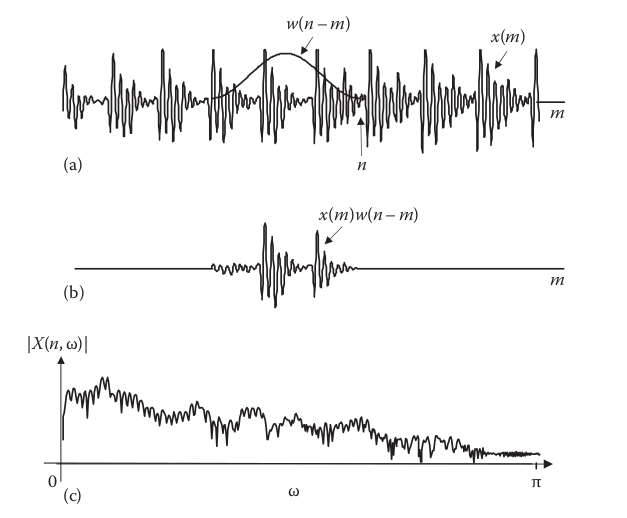
\includegraphics[scale=0.7]{images/ch2/stft_explained.png}}
	\caption{STFT como la transformada de Fourier de la señal $w[n-m] x[m]$. Imagen tomada de \cite{speech_enhancement_theory_and_practice}}
	\label{fig:ch2_stft_explained}
\end{figure}

Para la existencia de la STFT de $x[m]$ basta que la función $w[n-m]x[m]$ sea absolutamente sumable \cite{oppenheim_schafer} lo cual en general es cierto debido a la finita duración de $w[n-m]$

La STFT permitirá hacer un procesamiento de las señales de habla en el dominio de la frecuencia, sin embargo, una vez realizado será necesario volver al dominio del tiempo con lo que se necesitará la transformación inversa.

La secuencia $x[m]$ puede ser recuperada exactamente utilizando la ecuación de inversión de la transformada de Fourier

\begin{equation*}
	w[n-m] x[m] = \frac{1}{2 \pi} \int_{- \pi}^{\pi} X(n, \omega) e^{j \omega m}
\end{equation*}

Haciendo $m=n$ y suponiendo $\omega(0) \neq 0$, tenemos que:

\begin{equation*}
	x[n] = \frac{1}{2 \pi \omega(0)} \int_{- \pi}^{\pi} X(n, \omega) e^{j \omega m}
\end{equation*}

Esta inversión es conceptual, en la práctica se trabaja en forma discreta y se recurre a métodos alternativos que veremos en las próximas secciones.

\subsubsection{Muestreo en tiempo y frecuencia}
\label{sec:muestreo_en_tiempo_y_frecuencia}

Dado que el procesamiento de las señales de habla se realiza de forma digital, es necesario contar con la versión discreta de la STFT. Motivada por la definición de la DFT \cite{oppenheim_schafer}, se obtiene la versión discreta de la STFT por medio de muestrear la frecuencia en $N$ frecuencias separadas uniformemente en $\omega_k = \frac{2 \pi k}{N}$ con $k = 0, 1, ..., N$. Por lo tanto la versión discreta de la STFT queda definida como:

\begin{equation}
	STFT\{x[n]\}_{(n, \omega_k)} = X_{(n, \omega_k)} = \sum_{m=-\infty}^{\infty} x[m]w[n-m]e^{-j \omega_k m}
	\label{eq:stft_def}
\end{equation}

El proceso de ventanear la señal se podría repetir para cada $n$, es decir obtener la DFT de las secuencias: $w[0-m] x[m], w[1-m] x[m], w[2-m] x[m], ...$ para todo $n$. Esto resulta poco útil debido a que requiere mucho procesamiento y además se estaría obteniendo información redundante en el dominio de la frecuencia. Si bien las DFTs obtenidas serían distintas para cada una de las secuencias, la información espectral sería prácticamente la misma. Para evitar este procesamiento ineficiente se suele tomar una ventana cada R muestras de la señal $x[m]$, es decir se realiza un muestreo en tiempo. 

La STFT muestreada en el tiempo queda definida como:

\begin{equation}
	X_{(nR, \omega_k)} = \sum_{m=-\infty}^{\infty} x[m]w[nR-m]e^{-j \omega_k m}
	\label{eq:stft_def}
\end{equation}

Entonces, habrá tanto un muestreo en el dominio de la frecuencia como un muestreo en el dominio del tiempo, los cuales deben realizarse de tal manera que sea posible recuperar exactamente la señal $x[m]$.

De la DFT recordamos que para que no haya \emph{aliasing} en el dominio del tiempo se requiere que la variable de la frecuencia $\omega$ sea muestreada al menos $N$ veces para secuencias de largo $N$ \cite{oppenheim_schafer}. Dado que en nuestro caso las funciones $w[n-m] x[m]$ tiene largo $L$, tendremos el primer requerimiento que es $N \geq L$

Respecto de la elección del parámetro $R$, tendremos que si $R>L$, habrá ciertas muestras en el dominio del tiempo que se perderán, con lo cual se debe garantizar que $R \leq L$.

Estas dos condiciones llevan a la condición $R \leq L \leq N$ que de cumplirse permitirá recuperar la señal original $x[m]$. Estas condiciones son condiciones necesarias pero no suficientes. Dependiendo del tipo de método de reconstrucción que se utilice surgirán nuevas restricciones a cumplir. A continuación veremos el método de reconstrucción \emph{Overlapp-And-Add} el cual tiene la ventaja de ser estable numéricamente \cite{oppenheim_schafer}, lo cual resulta esencial en aplicaciones de reducción del ruido.

\subsubsection{El método de reconstrucción Overlapp-And-Add}
\label{sec:overlapp_and_and}

El presente método de reconstrucción se basa en la siguiente ecuación \cite{jae_sung_oppenheim}

\begin{equation*}
	\hat{x}[m] = \frac{R}{W(0)} \sum_{n=-\infty}^{\infty} \left[ \frac{1}{N} \sum_{k=0}^{N-1} X[mR, \omega_k] e^{j \omega_k n} \right]
\end{equation*}

donde 

\begin{equation*}
	W(0) = \sum_{m=-\infty}^{\infty} \omega[m]
\end{equation*}

El término entre corchetes no es más que la iDFT de las funciones $w[nR-m] x[m]$. Por lo tanto

\begin{align*}
	\hat{x}[m] &= \frac{R}{W(0)} \sum_{n=-\infty}^{\infty} w[nR-m] x[m] \\
	&= x(m) \frac{R}{W(0)} \sum_{n=-\infty}^{\infty} w[nR-m]
\end{align*}

Entonces para qué $\hat{x}[m] = x[m]$ se requiere que

\begin{equation*}
	\sum_{n=-\infty}^{\infty} w[nR-m] = \frac{W(0)}{R} = C
\end{equation*}

Esta es la restricción que impone el método \emph{Overlapp-And-Add} en la función ventana $\omega[m]$, la cual se reduce a que al sumar todas las ventanas, se obtenga la constante $C$. 

Es posible trabajar esta expresión para encontrar otras formas de expresar la restricción. Definimos la función  $\tilde{w}[m]$ como

\begin{equation*}
	\tilde{w}[m] = \sum_{n=-\infty}^{\infty} w[nR-m]
\end{equation*}

Esta función es periódica con periodo R con lo que se la puede escribir como iDFT de $W[\omega_k]$ con $k = 0, 1, ..., R-1$

\begin{equation*}
	\tilde{w}[m] = \frac{1}{R} \sum_{k=0}^{R-1} W[\omega_{k}] e^{j \omega_{k} m}
\end{equation*}

Si se cumpliese que $W[\omega_{k}]$ fuera 0 para $k = 1, 2, ..., R-1$ entonces se verificaría la condición original

\begin{equation*}
	\tilde{w}[m] = \sum_{n=-\infty}^{\infty} w[nR-m] = \frac{W[0]}{R}
\end{equation*}

Entonces, la condición equivalente del método \emph{Overlapp-And-Add} es que la DFT de la función ventana tenga ceros para $k = 1, 2, ..., R-1$.

Existen diversos tipos de funciones ventana, cada una con sus propiedades. Para el análisis de señales por medio de la STFT se requiere tener bajos niveles de fuga espectral \cite{speech_enhancement_theory_and_practice}, lo que lleva al uso de funciones ventanas como la ventana de Hann o su variante, la ventana de Hamming \cite{oppenheim_schafer}.

La función ventana de Hann tiene sus ceros en las frecuencias $4 k \pi/M$ con $M = L - 1$ \cite{oppenheim_schafer}, con lo que si estos ceros se alinean con los requeridos por el método, la condición de reconstrucción sin pérdidas estará verificada. Por lo tanto tenemos que:

\begin{equation*}
	\frac{2k\pi}{R} = \frac{4 k \pi}{M}
\end{equation*}

es decir, si elegimos $R$ tal que $R = M/2$, podremos reconstruir $x[m]$ sin pérdida de información.

\subsubsection{Espectrograma}
\label{sec:espectrograma}

La STFT es una función compleja. Una forma útil de analizar y de obtener información de las señales de habla es por medio del espectrograma que no es más que el módulo elevado al cuadrado de la STFT $|X_{(n, w)}^2|$. 

Usualmente el espectrograma es un gráfico en escala de colores o en escala de grises, donde a tonos más oscuros se tiene mayor energía para el tiempo y la frecuencia dados por los ejes x e y respectivamente. En la figura \ref{fig:ch2_spectrogram} podemos ver un ejemplo de una señal de habla junto a su espectrograma

\begin{figure}[H]
	\centering
	\centerline{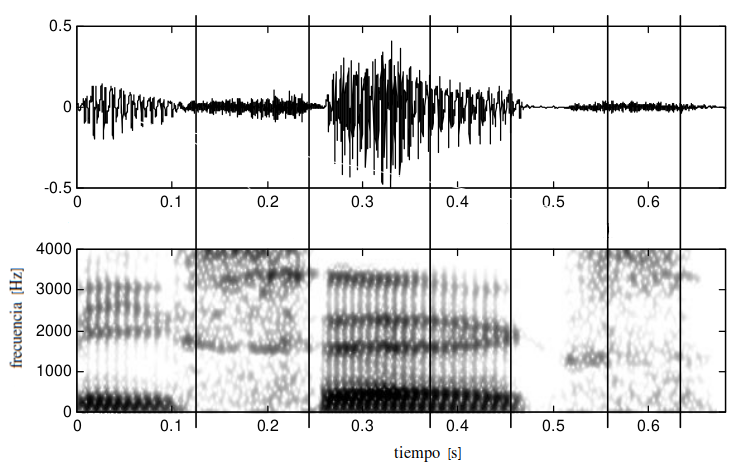
\includegraphics[scale=0.6]{images/ch2/spectrogram.png}}
	\caption{Señal de habla junto a su espectrograma. Imagen obtenida de \cite{spoken_language_processing}}
	\label{fig:ch2_spectrogram}
\end{figure}

La STFT permite captar cómo cambian las características espectrales de una señal en función del tiempo. A medida que aumenta la velocidad con la que cambian las características de una señal, más corta se tendrá que hacer la ventana utilizada en la STFT. Sin embargo, a medida que la ventana se hace más corta, se pierde resolución en frecuencia. Esto se debe a que en general el ancho del lóbulo principal de una función ventana es inversamente proporcional al largo de ella y este es el que principalmente determina la resolución en frecuencia.  Por ejemplo para la ventana de Hann y la de Hamming, el ancho del lóbulo principal es $8 \pi/L - 1$ \cite{oppenheim_schafer} 

Cuando se analizan señales de habla usando la STFT y en particular usando un espectrograma, es posible notar diferentes características de la señal de habla dependiendo del tamaño de ventana utilizado. En la figura \ref{fig:ch2_wideband_narrowband} podemos ver en (a) un espectrograma con una ventana de $\SI{24}{ms}$ y en (b) un espectrograma con una ventana de $\SI{8}{ms}$. 

\begin{figure}[H]
	\centering
	\centerline{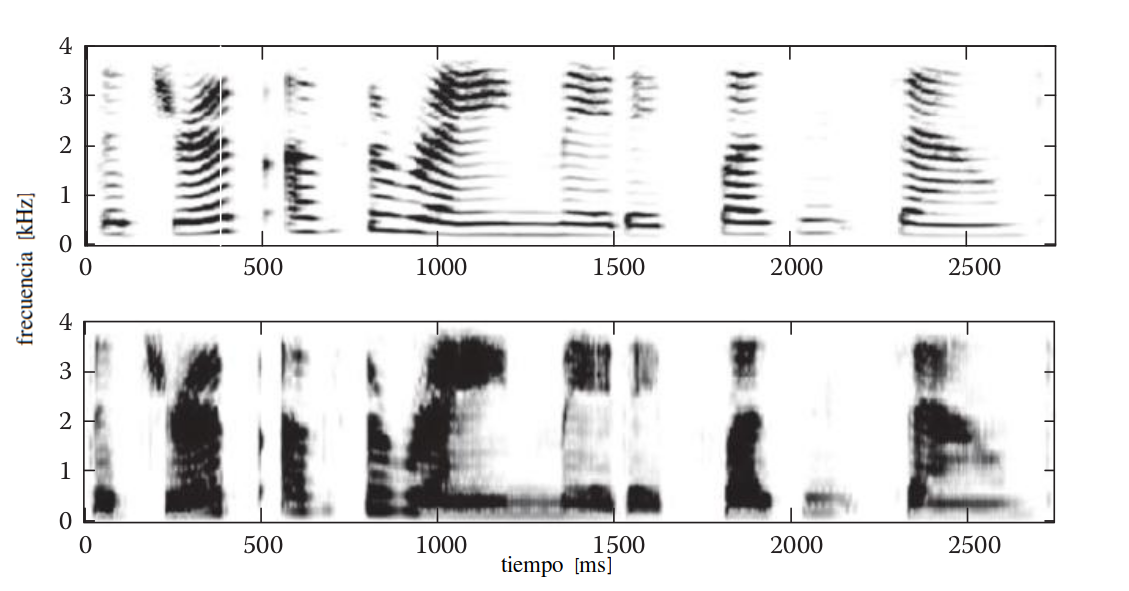
\includegraphics[scale=0.4]{images/ch2/wideband_narrowband.png}}
	\caption{Espectrograma de banda ancha y banda angosta. Imagen obtenida de \cite{speech_enhancement_theory_and_practice}}
	\label{fig:ch2_wideband_narrowband}
\end{figure}

Los espectrogramas con ventanas de largos mayores a los $\SI{20}{ms}$ se llaman espectrogramas de banda angosta y se caracterizan por tener buena resolución en frecuencia. Estos espectrogramas permiten por ejemplo resolver las frecuencias de resonancia y sus armónicas, generadas por el tracto vocal en sonidos vocálicos \cite{spoken_language_processing}. Esto se puede ver en la figura \ref{fig:ch2_wideband_narrowband} (a) donde las armonices aparecen como líneas horizontales.

Los espectrogramas con ventanas de largo menores a los $\SI{10}{ms}$ se llaman espectrogramas de banda ancha y se caracterizan por tener buena resolución en el dominio del tiempo. Esto permite por ejemplo poder detectar sonidos de corta duración como las consonantes oclusivas \cite{spoken_language_processing}. Sin embargo este tipo de espectrogramas oculta las armónicas como podemos ver en la figura \ref{fig:ch2_wideband_narrowband} (b) 

En lo que concierte a la reducción de ruido en señales de habla, en general se busca poder reconocer los distintos fonemas contenidos en las señales de habla, lo que lleva a optarse por ventanas de corto tiempo \cite{speech_enhancement_theory_and_practice}. Con ventanas cortas, tendremos una fina resolución en tiempo y resignaremos resolución en frecuencia.

\subsection{Sobre la importancia de la fase en las señales de habla} \label{sec:sobre_la_importancia_de_la_fase_en_las_señales_de_habla}

Usualmente los sistemas de supresión de ruido en señales de habla se basan en la estimación del espectrograma de la señal de habla, utilizando información presente en el espectrograma de la señal de habla ruidosa . 

Con esto lo que se pretende remarcar es que usualmente se estima únicamente la magnitud y no así la fase. En estos casos, la señal estimada se construye utilizando la magnitud estimada y la fase de la señal de habla ruidosa.

Es decir, dada la señal de habla ruidosa $x[n]$, su respectivo espectrograma $|X_{(n, w)}^2|$, su fase $\angle X_{(n, w)}$ y el espectrograma estimado de la señal de habla obtenida a la salida del filtro $|\hat{Y}_{(n, w)}^2|$, tenemos que:

\begin{equation*}
	\hat{Y}_{(n, w)} = |\hat{Y}_{(n, w)}| e^{i\angle X_{(n, w)}}
\end{equation*}

Esta suposición sobre la escasa importancia de la fase se basa en trabajos como el de Ohm sobre la ley de fase acústica \cite{ohm_s_law_of_acoustics} en el cual establece que la percepción de un tono de un sonido es una función de las amplitudes de las armónicas y no de la relación de fase entre ellas. 

Otros trabajos como \cite{the_unimportance_of_phase_in_speech_enhancement} realizaron estudios objetivos donde mezclaron magnitudes y fases a diferentes SNRs, esto les permitió obtener una SNR equivalente la cual en la mayoría de los casos estaba dominada por la SNR de la magnitud.

Esto lo que nos dice es que a la hora de diseñar un sistema para mejorar el nivel de ruido de una señal se debe prestar mayor atención a mejorar la SNR de la magnitud y no así la de la fase.


Si bien algunos estudios recientes como \cite{phase_importance_in_speech_processing_applications}, resaltan la importancia de contar con estimadores de calidad de la fase, en el presente trabajo se concentrará únicamente en la estimación de la magnitud.


\subsection{Restricciones de tiempo y procesamiento}
\label{sec:time_restrictions}

Como vimos en la sección \ref{sec:objetivos}, el presente trabajo se limita al estudio del filtrado de ruido en señales de habla para aplicaciones de videoconferencias. A la hora de desarrollar sistemas de filtrado de ruido, el objetivo final del sistema pondrá restricciones en su diseño. Un sistema de filtrado pensado para aplicaciones de videoconferencias debe ser un sistema causal y de tiempo real.

Que sea causal implica que las estimaciones realizadas por el sistema se realizarán únicamente basadas en información pasada. Que sea de tiempo real implica que el tiempo de procesamiento del sistema debe ser tal que no supere la latencia máxima aconsejable para sistemas de comunicación virtual.

Los sistemas de comunicación virtual emulan una comunicación cara-a-cara. Cuando se utiliza un filtro de ruido las etapas son:

\begin{itemize}
	\item Se recibe la señal de habla de un participante
	\item Se filtran los ruidos indeseables
	\item Se envía la señal filtrada a los demás integrantes.
\end{itemize}

El tiempo total desde que se emite la señal de habla hasta que llega a los demás, no debe superar ciertos umbrales. Según la recomendación de la Unión Internacional de Telecomunicaciones \cite{itu_t_recommendation_g_114}, los participantes de una reunión virtual comenzarán a notar el retraso a partir de los $\SI{100}{ms}$ y la conversación dejará de ser fluida aproximadamente a partir de los $\SI{250}{ms}$

\newpage

\section{Técnicas de filtrado de ruido en señales de habla}

\subsection{Ruidos estacionarios y no-estacionarios}

Los filtros de ruidos en señales de habla los podemos dividir en dos grupos. Por un lado, tenemos los filtros que permiten suprimir ruidos estacionarios y por otro lado, los que logran filtrar tanto ruido estacionario como no-estacionario.

Los filtros de ruidos estacionarios en señales de habla, en general, trabajan de la siguiente manera:

\begin{enumerate}
	\item Detectan períodos de no-habla.
	\item En el período de no-habla, estiman la magnitud del espectro del ruido.
	\item A la magnitud del espectro de la señal de habla ruidosa, le restan una estimación de la magnitud del espectro del ruido.
	\item Utilizando la fase de la señal ruidosa y la magnitud obtenida en el paso anterior, construyen la señal de habla filtrada.
\end{enumerate}

Este proceso tiene un inconveniente evidente. Para lograr un filtrado exitoso se requiere que el ruido no cambie durante los períodos de habla, es decir solo logra filtrar ruidos estacionarios.

Los ruidos no-estacionarios se caracterizan por ser de aparición espontánea, no periódica y usualmente de corta duración, haciendo sumamente compleja su correcta caracterización por medio de modelos matemáticos.

En las siguientes secciones veremos un repaso de las técnicas de filtrado de ruido estacionario y no-estacionario en señales de habla.

\subsection{Técnicas tradicionales de filtrado de ruido en señales de habla}

En la presente sección repasaremos algunas de las técnicas de filtrado comúnmente utilizadas para suprimir ruidos en señales de habla.

\subsubsection{Sustracción espectral}
\label{sec:sustraccion_espectral}

La técnica conocida como sustracción espectral, en su versión más básica, consiste en sustraer del espectro de la señal ruidosa una estimación del espectro del ruido obtenido en periodos de no habla.

Formalmente, dada la señal de habla ruidosa $y(n)$, la señal de habla sin ruido $x(n)$ y el ruido aditivo $d(n)$ tenemos que:

\begin{equation*}
	y(n) = x(n) + d(n)
\end{equation*}

Tomando la DFT de ambos lados:

\begin{equation*}
	Y(\omega) = X(\omega) + D(\omega)
\end{equation*}

y por lo tanto:

\begin{equation*}
	X(\omega) = Y(\omega) - D(\omega)
\end{equation*}

lo cual se puede descomponer en:

\begin{equation*}
	|X(\omega)| = |Y(\omega) - D(\omega)| \qquad \text{y} \qquad \phi_{X(\omega)} = \phi_{Y(\omega) - D(\omega)}
\end{equation*}

Suponiendo que la fase de $Y(\omega)$ es aproximadamente colineal a la fase de $D(\omega)$ se obtiene que:

\begin{equation*}
	|\hat{X}(\omega)| = |Y(\omega)| - |D(\omega)| \qquad \text{y} \qquad \hat{\phi}_{X(\omega)} = \phi_{Y(\omega)}
\end{equation*}

Donde la magnitud de la señal de ruido $D(\omega)$ se estima en los periodos de no-habla.

Un problema evidente que surge a partir de las aproximaciones realizadas, es que la resta $|Y(\omega)| - |D(\omega)|$ puede llevar a un valor negativo de $|\hat{X}(\omega)|$. En la práctica usualmente lo que se hace es implementar un rectificador de media onda, es decir:

\begin{equation*}
	|\hat{X}(\omega)| = \begin{cases} 
		|Y(\omega)| - |D(\omega)| & \text{si} \quad |Y(\omega)| >  |\hat{D}(\omega)| \\
		0 & \text{si} \quad |Y(\omega)| \leq  |\hat{D}(\omega)|\\
	\end{cases}
\end{equation*}

La señal de habla mejorada se obtiene simplemente tomando la iDFT, es decir:

\begin{equation*}
	\hat{x}(n) = iDFT \left\{ |\hat{X}(\omega)| e^{\phi_{Y(\omega)}} \right\}
\end{equation*}

La no linealidad introducida por el rectificador generan, en el dominio del tiempo, unos picos que son perceptibles para el oído humano, a dicho ruido se lo conoce como ruido musical. En ocasiones este ruido introducido por la sustracción espectral puede resultar en un sonido incluso más desagradable que el generado por el ruido aditivo.

Por lo tanto, el método de sustracción espectral es relativamente sencillo de implementar, pero trae principalmente dos problemas:

\begin{enumerate}
	\item El ruido musical generado por el rectificador de media onda.
	\item La necesidad de contar con pausas en la señal de habla para una correcta estimación de $|D(\omega)|$.
\end{enumerate}

Si bien existen técnicas para combatir los problemas (1) y (2) \cite{speech_enhancement_theory_and_practice}, los sistemas resultantes terminan siendo complejos de llevar a la práctica.

\subsubsection{Filtro de Wiener}

El método de sustracción espectral aprovecha la característica aditiva del ruido para obtener la señal de habla filtrada por medio de restar una estimación de la magnitud del ruido. Este método, si bien es efectivo, resulta no ser óptimo en el sentido del error cuadrático medio. 

El filtro de Wiener, aplicado al filtrado de ruidos en señales de habla, permite obtener un filtro óptimo utilizando el criterio del error cuadrático medio. 

Dada una señal objetivo $d(n)$, la señal a filtrar $y(n)$ y el siguiente sistema:


\begin{figure}[H]
	\centering
	\centerline{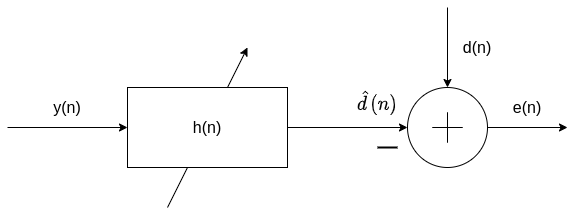
\includegraphics[scale=0.6]{images/ch3/wiener.png}}
	\caption{Filtro de Wiener.}
	\label{fig:ch3_wiener_filter}
\end{figure}


El filtro óptimo, en el sentido del error cuadrático medio, viene dado por:

\begin{equation*}
	h_{opt} = R_{yy}^{-1} R_{dy}
\end{equation*}

\noindent donde $R_{yy}$ es la matriz de autocorrelación del proceso $y$, y $ R_{dy}$ es el vector de correlación cruzada entre el proceso $y$ y la variable aleatoria $d$.

Por otro lado, si consideramos, nuevamente un ruido aditivo:

\begin{equation*}
	y(n) = x(n) + n(n)
\end{equation*}

\noindent tendremos que el filtro óptimo viene dado por \cite{speech_enhancement_theory_and_practice}:

\begin{equation*}
	h_{opt} = \left( R_{xx} + R_{nn} \right)^{-1} R_{xx}
\end{equation*}

\noindent o en el dominio de la frecuencia \cite{speech_enhancement_theory_and_practice}:

\begin{equation*}
	H(\omega) = \frac{P_{xx}(\omega)}{P_{xx}(\omega) + P_{nn}(\omega)}
\end{equation*}

\noindent donde P es la densidad espectral de potencia. Dado

\begin{equation*}
	X(\omega) = DTFT\{ x_{(n)} \} \qquad \text{y} \qquad N(\omega) = DTFT\{ n_{(n)} \}
\end{equation*}

\noindent entonces, la densidad espectral de potencia viene dada por \cite{intuitive_probability_and_random_processes_using_matlab}:

\begin{equation*}
	P_{xx} = E[ | X(\omega) |^2 ] \qquad \text{y} \qquad P_{nn} = E[ | N(\omega) |^2 ]
\end{equation*}

Conocido ya el filtro óptimo en el sentido del error cuadrático medio, el siguiente problema a resolver es la estimación de las densidades $P_{xx}$ y $P_{nn}$ o las respectivas funciones de auto-correlaciones.

Una de las técnicas utilizadas en la práctica consiste en modelar la señal de habla como la respuesta de un sistema LTI, como el que se muestra en la figura \ref{fig:ch3_voice_modeling} \cite{spoken_language_processing}. 

Los sonidos del tipo vocálicos son modelados con una excitación periódica y los del tipo no-vocálicos modelados con una excitación aleatoria. El sistema LTI modela el tracto vocal y a la salida del sistema se obtiene la señal de habla.

\begin{figure}
	\centering
	\centerline{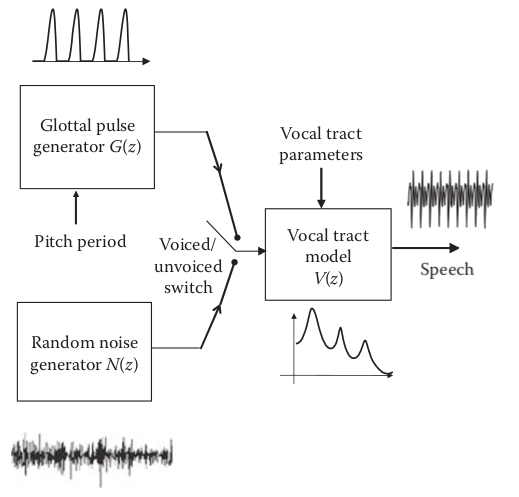
\includegraphics[scale=0.5]{images/ch3/voice-modeling.png}}
	\caption{Modelo de las señales de habla. Imagen tomada de \cite{speech_enhancement_theory_and_practice}.}
	\label{fig:ch3_voice_modeling}
\end{figure}


Al tracto vocal usualmente se lo modela como un sistema formado únicamente por polos \cite{spoken_language_processing}, con lo que $V(z)$ tiene una transformada Z de la forma:

\begin{equation*}
	V(z) = \frac{q}{1 - \sum_{k=1}^{p} a_k z^{-k}}
\end{equation*}

Por lo tanto, en el dominio del tiempo, la señal de habla responde a la ecuación diferencial:

\begin{equation*}
	x(n) = \sum_{k=1}^{p}a_k x(n-k) + g \; u(n)
\end{equation*}

\noindent donde $u(n)$ representa la excitación.

Estimados los coeficientes $a_k$ se podría obtener la densidad espectral de potencia $P_{xx}$ y con ello obtener el filtro óptimo. En \cite{all_pole_modeling_of_degraded_speech} utilizan la técnica de máximo a posteriori para estimar los coeficientes $a_k$

A diferencia de la sustracción espectral, en este caso no fue necesario utilizar los momentos de pausa para estimar la magnitud del espectro del ruido, pero si se requirió la utilización de modelos para la señal de voz y modelos para el ruido aditivo. 

En algunos casos de usos se puede obtener un filtro de ruidos en señales de habla con un buen desempeño, pero cuando las condiciones reales se alejan del modelo, el sistema comienza a fallar, lo que sucede especialmente con el modelo del ruido.

\subsection{Técnicas de filtrado de ruido en señales de habla basadas en filtros adaptativos}
\label{sec:adaptive_filter}

\subsubsection{Arquitectura de un filtro adaptativo como cancelador de ruido}
\label{sec:adaptive_filter_architecture}

En algunas aplicaciones resulta posible la utilización de más de un micrófono para captar las señales de habla. En estos casos resulta posible la utilización de un filtro adaptativo \cite{fundamentals_of_adaptive_filtering}.

Usualmente en este tipo de situaciones se tiene un micrófono, el cual capta la señal de habla más el ruido aditivo y por otro lado, un micrófono que capta únicamente el ruido.

A continuación podemos ver la configuración de un cancelador de ruido basado en un filtro adaptativo:

\begin{figure}[H]
	\centering
	\centerline{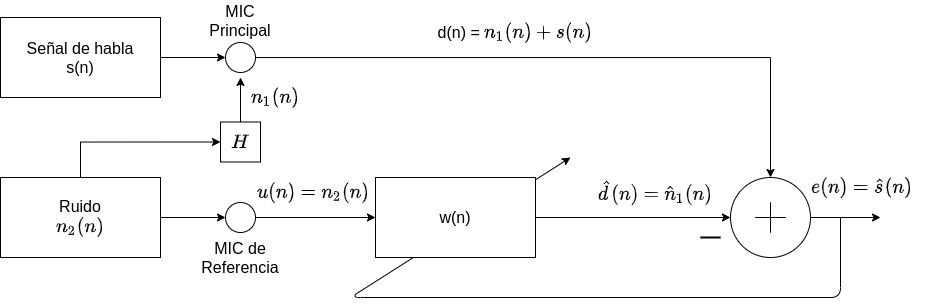
\includegraphics[scale=0.5]{images/ch3/af-se-setup.png}}
	\caption{Filtro adaptativo configurado como cancelador de ruido. Imágen tomada de \cite{a_family_of_adaptive_filter_slgorithms_in_noise_cancellation_for_speech_enhancement}.}
	\label{fig:ch3_af-se-setup}
\end{figure}

El micrófono principal captura la señal de habla $s(n)$ corrompida por el ruido $n_1(n)$ . Por otro lado, el micrófono de referencia captura la señal de ruido $n_2(n)$, el cual está correlacionado con el ruido $n_1(n)$. 

El ruido $n_2(n)$ pasa por el filtro adaptativo, el cual lo transforma para obtener una estimación del ruido $n_1(n)$. Al restar la señal de habla ruidosa, con una estimación del ruido que la corrompió originalmente, es posible obtener una estimación de la señal de habla. 

Este modelo supone que existe un filtro $H$, el cual transforma el ruido $n_2(n)$ en $n_1(n)$. Dada la configuración de la figura \ref{fig:ch3_af-se-setup}, el filtro adaptativo tratará de estimar los coeficientes del filtro $H$. El buen desempeño del filtro estará principalmente dado por la exactitud con la que logre aproximar a $H$.

El filtro se auto-ajusta continuamente, de manera tal que se minimice el error cuadrático medio entre $n_1(n)$ y $\hat{n}_1(n)$ . La señal de error viene dada por:

\begin{equation*}
	e(n) = \hat{s}(n) = n_1(n) + s(n) - \hat{n}_1(n)
\end{equation*}

\noindent calculando el valor esperando de ambos lados:

\begin{align*}
	\mathbb{E}[e^2] &= \mathbb{E}[( n_1 + s - \hat{n}_1)^2] \\ \\
	&= \mathbb{E}[n_1^2 + s^2 + \hat{n}_1^2 - 2 n_1 s - 2 \hat{n}_1 n1]
\end{align*}

Si la señal de habla se encuentra descorrelacionada con los ruidos $n_1$ y $n_2$, y además ambos ruidos están correlacionados entre sí, es decir:

\begin{equation*}
	\mathbb{E}[n_1 s] = 0 \qquad \mathbb{E}[n_2 s] = \mathbb{E}[\hat{n}_1 s] = 0 \qquad \mathbb{E}[n_1 n_2] \neq 0
\end{equation*}

\noindent obtenemos que:

\begin{align*}
	\mathbb{E}[e^2] = \mathbb{E}[s^2] + \mathbb{E}[(n_1 - \hat{n}_1)^2]
\end{align*}

Por lo que el filtro, al minimizar $\mathbb{E}[( n_1 + s - \hat{n}_1)^2]$, también minimiza $\mathbb{E}[(n_1 - \hat{n}_1)^2]$.


\subsubsection{Filtro RLS}
\label{sec:adaptive_filter_rls}

En la sección anterior vimos la arquitectura de un filtro adaptativo utilizado para filtrar ruidos en señales de habla. Además de definir la configuración del filtro es necesario establecer la regla de optimización. Alguno de los algoritmos mas comúnmente utilizados son \cite{a_family_of_adaptive_filter_slgorithms_in_noise_cancellation_for_speech_enhancement}; el LMS, el NLMS, el RLS y el APA.

En \cite{a_family_of_adaptive_filter_slgorithms_in_noise_cancellation_for_speech_enhancement} podemos ver que, entre los algoritmos evaluados, el RLS es el que logra el menor error cuadrático medio y el que tiene mayor velocidad de convergencia. En base a estos resultados se decidió limitar el presente trabajo a la utilización del algoritmo RLS. 

El algoritmo RLS describe la solución recursiva al problema de cuadrados mínimos ponderado y regularizado definido por \cite{fundamentals_of_adaptive_filtering}:

\begin{equation*}
	\min_{ \omega} \left[\lambda^{N+1} \omega^* \Pi \omega + \sum_{j=0}^N \lambda^{N-j} |d(j) - u_j \omega |^2 \right]
\end{equation*}

\noindent donde $ 0 \ll \lambda \leq 1$ es el factor de olvido, el cual selecciona qué tanta importancia se le debe dar a las muestras pasadas. 

Desde el punto de vista de los filtros adaptativos, el algoritmo RLS surge a partir de aproximar las matrices de autocorrelación de los procesos $d$ y $u$ para lograr aproximar el gradiente de la función de costo $J(\omega) = \mathbb{E} | d - u \omega |^2$.

El filtro óptimo viene dado por medio de la ecuación de Wiener:

\begin{equation*}
	w^o = R_u^{-1}R_{du}
\end{equation*}

Utilizando la técnica de gradiente descendiente se obtiene la recursión:

\begin{equation*}
	w_i = w_{i-1} - \mu(i) \left[ \nabla^2_\omega J(\omega_{i-1}) \right] \left[ \nabla_w J(w_{i-1}) \right]^*
\end{equation*}

\noindent la cual puede reducirse a \cite{fundamentals_of_adaptive_filtering}:

\begin{equation*}
	w_i = w_{i-1} + \mu(i) (\epsilon(i) I + R_{uu} )^{-1} \left( R_{du} - R_{uu} w_{i-1} \right)
\end{equation*}

Como en la práctica no se suele conocer las matrices de autocorrelación $R_u$ y $R_{du}$, éstas son aproximadas. Para el caso del filtro RLS las aproximaciones utilizadas vienen dadas por:

\begin{equation*}
	\hat{R}_{du} = u_i^* d(i) \qquad \text{y} \qquad \hat{R}_{uu} = \frac{1}{i+1} \sum_{j=0}^{i} \lambda^{i-j} u_j^* u_j
\end{equation*}

Para $R_u$ se está usando el estimador de media muestral incluyendo el factor de olvido $\lambda$ y para $\hat{R}_{du}$ se están utilizando los valores instantáneos.

\subsubsection{Error en estado estacionario}
\label{sec:adaptive_filter_stationary_error}

Como vimos en la sección anterior, los filtros adaptativos buscan minimizar la función de costo $J(\omega) = \mathbb{E} | d - u \omega |^2$. La solución óptima en el sentido del error cuadrático medio es \cite{fundamentals_of_adaptive_filtering}:

\begin{equation*}
	w^o = R_u^{-1}R_{du}
\end{equation*}

Entonces el mínimo error vendrá dado por $J(w_o)$, el cual se puede probar que es \cite{fundamentals_of_adaptive_filtering}:

\begin{equation*}
	J_{min} = J(w_o) = \sigma_d^2 - R_{ud} R_{u}^{-1} R_{du}
\end{equation*}

Es decir, en el caso de tener caracterizados los procesos estocásticos y contar con la matrices de autocorrelación, el error de aproximación de la señal $d(n)$ será mayor o igual a $J_{min}$. Para el caso donde no se cuenta con estas matrices y se recurra a aproximaciones como en el algoritmo RLS, el error va a ser aún mayor, ya que las aproximaciones estocásticas introducen ruido en la estimación del gradiente \cite{fundamentals_of_adaptive_filtering}.

\subsubsection{Procesamiento de las señales de habla}
\label{sec:filtro_adaptativo_procesamiento_de_señales}

Los filtros adaptativos trabajan de forma recursiva, es decir, para obtener la salida en el tiempo $n$ se necesita el estado del filtro en el tiempo $n-1$ y las señales $d(n)$ y $u(n)$. 

Utilizando las aproximaciones de $R_u$ y $R_{du}$ vistas en la sección anterior y definiendo:

\begin{equation*}
	\mu(i) = \frac{1}{i+1} \qquad \text{y} \qquad \epsilon(i) = \frac{\lambda^(i+1) \epsilon}{i + 1}
\end{equation*}

se puede obtener la siguiente recursión \cite{fundamentals_of_adaptive_filtering}:

\begin{equation*}
	w_i = w_{i-1} + P_i u_i^* \left( d(i) - u_i w_{i-1} \right)
\end{equation*}

donde:

\begin{equation*}
	P_i = \lambda^{-1} \left(P_{i-1} - \frac{\lambda^{-1} P_{i-1} u_i^* u_i P_{i-1}}{1 + \lambda^{-1} u_i P_{i-1} u_i^*} \right)
\end{equation*}

con la condición inicial $P_{-1}=\epsilon^{-1}$ y $ 0 \ll \lambda \le 1$.

El procesamiento de una señal de habla consiste en los siguientes pasos:

\begin{enumerate}
	\item Inicializar los coeficientes del filtro.
	\item Usando $d(i)$ y $u(i)$, obtener $P_i$ y $w_i$.
	\item Obtener la señal de habla filtrada dada por la señal $e(i) = d(i) - u_i w_i $.
	\item Volver al paso 2.
\end{enumerate}

\subsection{Técnicas de filtrado de ruido en señales de habla basadas en redes neuronales}
\label{sec:tecnicas_filtrado_redes_neuronales}

La limitante que poseen los filtros adaptativos es la necesidad de contar con una señal de referencia, lo cual conlleva a la necesidad de utilizar múltiples micrófonos. En algunos casos de usos, tal requerimiento es incluso prohibitivo lo cual impulsa la búsqueda de nuevas soluciones. 

Como vimos en la sección \ref{sec:sustraccion_espectral}, una técnica comúnmente utilizada para filtrar señales de habla corrompidas por ruido, es la técnica de sustracción espectral. Esta técnica, consiste en obtener una estimación del espectro del ruido durante los periodos de silencio. El espectro estimado se usa para filtrar la señal de habla corrompida. Una desventaja de esta técnica es que si el ruido es no-estacionario, la variabilidad del mismo no permite mantener una correcta estimación del espectro del ruido.

En la última década, el gran avance que hubo en el desarrollo de redes neuronales \cite{deep_learning} permitió elaborar redes capaces de filtrar señales de habla corrompidas incluso en casos de uso donde solo se cuenta con la información provista por un solo micrófono. 

A diferencia de la sustracción espectral o de los filtros adaptativos que se basan en la utilización de técnicas de procesamiento de señales, el filtro basado en redes neuronales es una técnica basada en datos. Es decir, para poder desarrollar estos filtros se necesitan de una gran cantidad de señales corrompidas que permitan entrenar la red de manera que los parámetros de la misma se ajusten de forma tal que se minimice la diferencia entre las señales filtradas y las señales de habla sin ruido.

\subsubsection{Información de entrada y de salida}

Se ha demostrado que el tipo de información que resulta más relevante para entrenar este tipo de redes, es la potencia espectral logarítmica \cite{a_regression_approach_to_speech_enhancement_based_on_deep_neural_networks}. 

Haciendo una simplificación, podemos pensar que como entrada de la red, se usa el espectro de la señal corrompida por ruido y a la salida, como señal objetivo, se usa el espectro de la señal original, de manera que la red aprenda a realizar las transformaciones necesarias para llegar de una señal a la otra.

Dado que las señales de habla ruidosas son no-estacionarias es necesario analizarlas por tramos, por tal motivo resulta conveniente la utilización de la transformada de Fourier de tiempo corto STFT. 

Dada la señal de habla ruidosa $d[n]$, la información utilizada para entrenar la red es:

\begin{equation*}
	X(n, w) = log(|STFT\{d[n]\}|^2) = log(|D(n, w)|^2)
\end{equation*}

Por otro lado la señal objetivo sera $s[n]$, por lo tanto la información utilizada a la salida será:

\begin{equation*}
	Y(n, w) = log(|STFT\{s[n]\}|^2) = log(|S(n, w)|^2)
\end{equation*}

Dado que se requiere construir un filtro de ruido para aplicaciones de tiempo real, resulta necesario obtener $Y(n, w)$ usando únicamente la señal de habla ruidosa hasta el tiempo $n$, es decir $\{..., X(n - 2, w), X(n - 1, w), X(n, w)\}$. 

Hay otras aplicaciones que no requieren un procesamiento en tiempo real de la señal de habla, donde para obtener $Y(n, w)$ se podría utilizar tanto información pasada como información futura. Por ejemplo, una aplicación de separación de habla se encarga de tomar una señal de audio mezclada y separarla en las distintas fuentes que la produjeron. Esta aplicación no requiere que se realice el procesamiento en tiempo real. Para obtener $Y(n, w)$ se puede usar tanto información pasada $\{..., X(n - 2, w), X(n - 1, w), X(n, w)\}$ como futura $\{X(n +1, w), X(n + 2, w), ...\}$. 

Usualmente se trabajan con 3 tipos de estructuras de redes en las aplicaciones de cancelación de ruido en señales de habla \cite{a_regression_approach_to_speech_enhancement_based_on_deep_neural_networks,a_fully_convolutional_neural_network_for_speech_enhancement,a_convolutional_recurrent_neural_network_for_real_time_speech_enhancement}:

\begin{enumerate}
	\item Feedforward
	\item Convolucionales
	\item Recurrentes
\end{enumerate}

\subsubsection{Redes neuronales del tipo feedforward}

Las redes del tipo feedforward \cite{deep_learning} son una de las estructuras de red más simples que se puede utilizar como filtro de ruido en señales de habla. 

Las redes neuronales feedforward consisten, usualmente, en una serie de capas, cada una con un conjunto de parámetros los cuales se auto-ajustan durante el entrenamiento de manera tal de generar cierta transformación.

Dada la potencial espectral logarítmica de la señal de habla ruidosa $X(n, w)$, la potencial espectral logarítmica de la señal de habla sin ruido $Y(n, w)$ y definiendo un modelo de red neuronal con suficiente capacidad de aprendizaje, se espera que la red neuronal sea capaz de encontrar una función que permita realizar la transformación $X(n, w) \longrightarrow Y(n, w)$.

Los espectrogramas $X(n, w)$ e $Y(n, w)$ son función de 2 variables, el tiempo y la frecuencia. Las redes neuronales feedforward pueden procesar información unidimensional, con lo que la generación de $Y(n, w)$ no es inmediata. Recordemos de la sección \ref{sec:stft} que $X(i,w)$ en el dominio del tiempo representa una ventana de la señal $x(m)$. 

\begin{figure}
	\centering
	\centerline{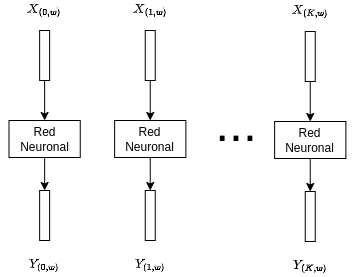
\includegraphics[scale=0.7]{images/ch3/features-ffnn.png}}
	\caption{Procesamiento de espectrogramas con una red del tipo feedforward.}
	\label{fig:ch3_features_ffnn}
\end{figure}

Una forma de procesar, con la red neuronal, la matriz $X(n, w)$, es armar vectores formados por J filas, con la forma $[X(i-J+1,w), X(i-J+2,w), ... , X(i,w)]$. Donde $J$ es la cantidad de ventanas hacia atrás del tiempo $i$ que se utilizan para determinar $Y(i, w)$. 

En la figura \ref{fig:ch3_features_ffnn} podemos ver el proceso para obtener $Y(i, w)$, el cual consta de hacer pasar por la red los vectores $[X(i, w), X(i+1, w), ..., X(i+J-1, w)]$. Por cada vector de entrada, se obtiene, a la salida de la red, el vector $Y(i, w)$. Agrupando todas las salidas finalmente se obtiene $Y(n, w)$.

Uno de los problema de esta solución, es que la dimensión del vector de entrada crece rápidamente a medida que $J$ se hace mas grande. Cada vector $X(i, w)$ tiene un tamaño de $N/2$ muestras, donde $N$ es la cantidad de muestras utilizados en la $DFT$ de $x(m) \omega(nR-m)$. Entonces, por ejemplo, para $N=1024$ y $J=32$, tendríamos un vector de entrada de dimensión $512 \cdot 32 = 16384$. Otro de los problemas con este enfoque, es que la salida $Y(i, w)$, queda como un función de todos los puntos del vector de entrada, algo que esta lejos de representar correctamente las dependencias temporales existentes en las señales de habla.

\subsubsection{Redes neuronales del tipo convolucionales}
\label{sec:redes_convolucionales}

Una de las estructuras de redes neuronales que permite procesar información n-dimensional y aprender características locales, son las redes convolucionales \cite{deep_learning}. 

Las redes convolucionales están formadas por capas convolucionales, las cuales poseen una serie de filtros o \emph{kerneles}. Estos filtros se adaptan durante el entrenamiento de manera tal que se pueda obtener características locales, abarcando las n dimensiones.

A diferencia de las redes \emph{feedforward} donde para procesar la matriz:

\begin{equation*}
	\{X(i, w), X(i+1, w), ..., X(i+J-1, w)\}
\end{equation*}

\noindent es necesario desarmarla y formar un vector. Con la red convolucional, se la puede procesar sin modificación alguna. En la figura \ref{fig:ch3_features_cnn}, podemos ver el proceso para obtener $Y(n, w)$ a partir de $X(n, w)$.

\begin{figure}
	\centering
	\centerline{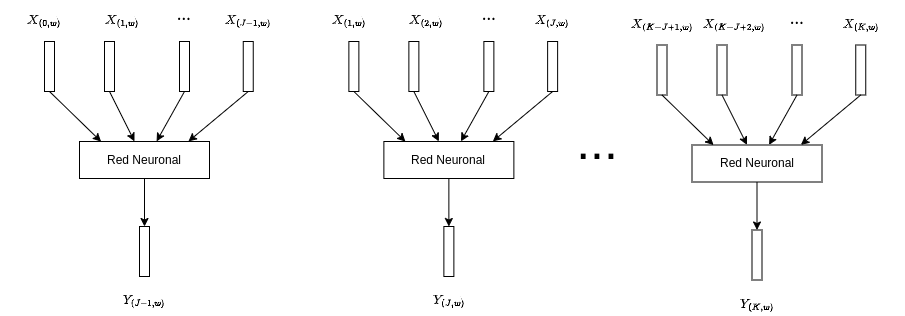
\includegraphics[scale=0.5]{images/ch3/features-cnn.png}}
	\caption{Procesamiento de espectrogramas con una red del tipo convolucional.}
	\label{fig:ch3_features_cnn}
\end{figure}

\subsubsection{Redes neuronales auto-codificadoras}
\label{sec:redes_autocodificadoras}

El diseño de una arquitectura de red neuronal involucra múltiples factores. Uno de ellos es la elección del tipo de capa a utilizar. Como vimos en la sección anterior, algunos de los tipos de capas que se pueden utilizar son las capas feedforward o las capas convolucionales. 

Otro de los factores a diseñar es cómo la arquitectura logrará cumplir el objetivo final, el cual en nuestro caso es el de reducir el ruido en las señales de habla. Una de las arquitecturas de redes que tiene esta característica son las redes auto-codificadoras.

Una red auto-codificadora es un tipo de red entrenada para generar una copia de la entrada \cite{deep_learning}. Como se muestra en la figura \ref{fig:ch3_autoencoder}, la red se puede dividir en dos, una función codificadora $h=f(x)$ y una función decodificadora $r=g(h)$. En conjunto, ambas partes aprenden la identidad $g(f(x)) = x$.

Una de las aplicaciones más comunes es la de utilizarla como una reductora de la dimensión de entrada. Cuando a una red auto-codificadora se la entrena para reducir la dimensión de entrada, se la fuerza a capturar las características más importantes del conjunto de entrenamiento.

\begin{figure}
	\centering
	\centerline{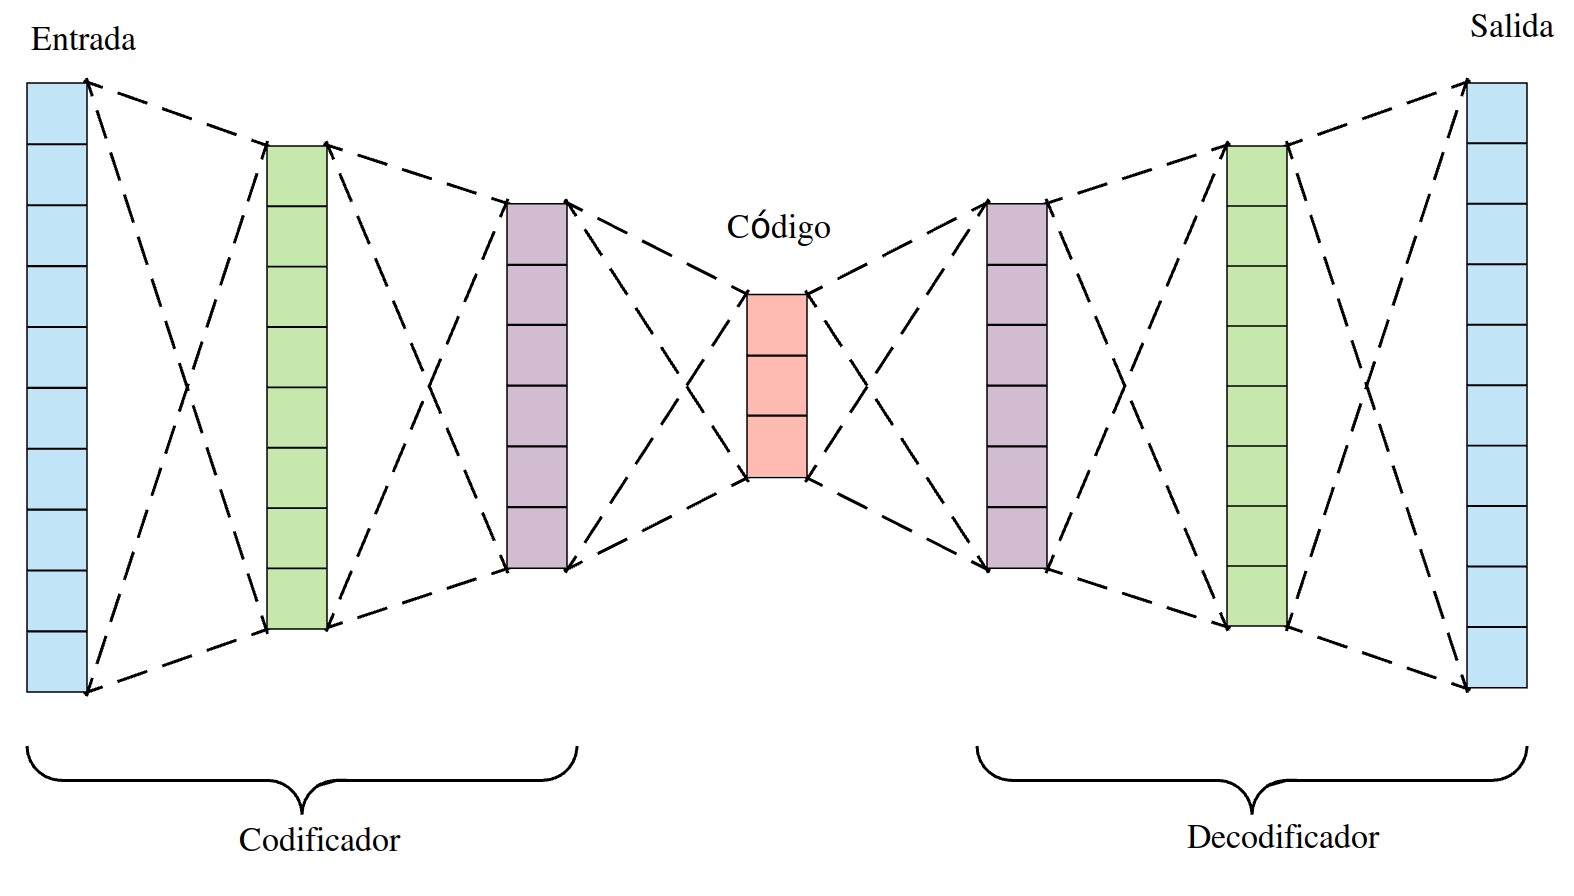
\includegraphics[scale=0.2]{images/ch3/autoencoder.png}}
	\caption{Red neuronal del tipo auto-codificadora.}
	\label{fig:ch3_autoencoder}
\end{figure}

El objetivo del codificador es reducir el tamaño de las señales, de forma tal que al ser decodificadas, la señal resultante minimice cierta función de error respecto de la señal original. Generalmente la función de error utilizada es el error cuadrático medio.

Otra de las funciones comunes de las redes auto-codificadoras es la de remover ruido. A la entrada del codificador se presentan las señales ruidosas y a la salida las señales filtradas. Con esto el auto-codificador aprende a generar la señal filtradas, utilizando la menor cantidad de información posible y por ende aprende a mantener la información relevante de la señal y descartar el ruido.

\subsubsection{Redes neuronales auto-codificadoras con estructura del tipo U}
\label{sec:redes_tipo_u}

La arquitectura del tipo U se usó por primera vez en un trabajo de segmentación de imágenes bio-médicas \cite{U_Net_Convolutional_Networks_for_Biomedical_Image_Segmentation}. En este tipo de tareas la red debe aprender a asignar una etiqueta a cada píxel de la imagen de entrada. Para logarlo, se necesita un modelo de red neuronal capaz de trabajar con gran precisión y localización, es decir trabajar a nivel de un píxel y capaz de localizar áreas con gran exactitud.

Estas características de las redes del tipo U hacen que sean efectivas para trabajar en el dominio de la STFT, donde un desplazamiento en tiempo o en frecuencia afecta considerablemente la calidad y la inteligibilidad de los sonidos. En \cite{singing_voice_separation_with_deep_u_net_convolutional_networks} este tipo de arquitectura fue utilizada para una aplicación de separación de fuentes en señales de audio.

La arquitectura del tipo U consta de un codificador y un decodificador. En la figura \ref{fig:ch3_unet} podemos ver el codificador en los bloques de la izquierda y el decodificador en los bloques de la derecha.

\begin{figure}
	\centering
	\centerline{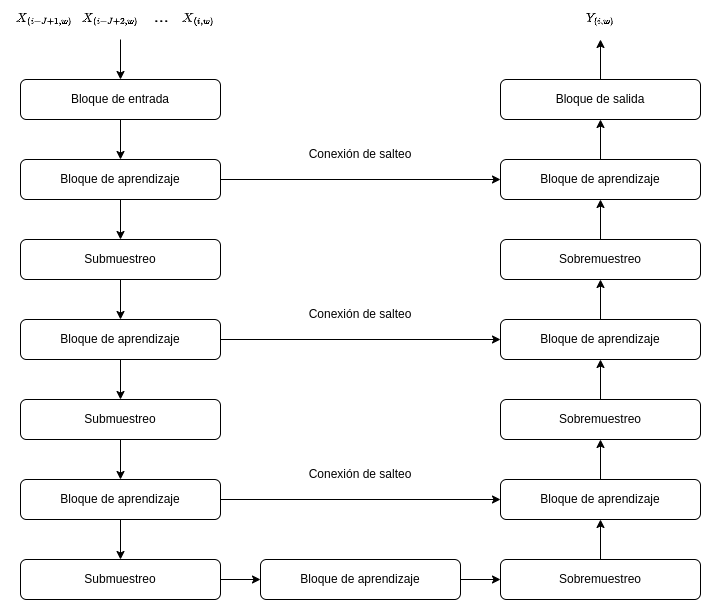
\includegraphics[scale=0.65]{images/ch3/unet.png}}
	\caption{Red neuronal auto-codificadora del tipo U.}
	\label{fig:ch3_unet}
\end{figure}

El codificador de la red consiste en el camino contractivo, el cual se encarga de reducir la dimensión. Esto lo logra por medio de:

\begin{enumerate}
	\item Un bloque de aprendizaje, que se encarga de aprender atributos locales. Estos bloques son esencialmente convolucionales. Aumentan la cantidad de canales de la señal de entrada, permitiendo ajustar los filtros de tal manera que cada nivel aprende a distinguir ciertos rasgos de la señal de entrada.
	
	\item Un bloque de sub-muestreo que reduce a la mitad la dimensión de su entrada. La reducción la logra por medio de la ejecución de operaciones de agrupación por máximo valor (\emph{max pooling} \cite{deep_learning}). La operación de agrupación por máximo valor es esencial para que se mantengan los atributos relevantes y se descarten los restantes.
\end{enumerate}

El decodificador de la red consiste en el camino expansivo. Realiza la tarea opuesta al camino contractivo, es decir, aumenta la dimensión, nuevamente con un bloque de aprendizaje y con un bloque de sobre-muestreo:


\begin{enumerate}
	\item Nuevamente el bloque de aprendizaje se encarga de obtener atributos relevantes. En lugar de aumentar la cantidad de canales de la señal de entrada los reduce, permitiendo recuperar la señal de entrada sin los rasgos indeseables.
	
	\item Un bloque de sobre-muestreo que aumenta al doble la dimensión de su entrada. El aumento lo logra por medio de la ejecución de operaciones de interpolación.
\end{enumerate}

Además, a la salida de los bloques de aprendizaje tenemos una conexión de salteo. Estas conexiones permiten al camino expansivo recuperar características de la señal original. 

Los bloques de aprendizaje del camino expansivo reciben una entrada compuesta por; la salida del bloque anterior junto con la concatenación de la salida del bloque de aprendizaje del camino contractivo. Esto les permite operar con el doble de información \cite{the_importance_of_skip_connections_in_biomedical_image_segmentation}.

Veamos cómo se componen cada uno de los bloques de la figura \ref{fig:ch3_unet}. El bloque de entrada está compuesto por:

\begin{itemize}
	\item Una capa convolucional con un núcleo de tamaño 3x3, un paso de 1 y un rellenado de 1. Esta combinación de parámetros permite obtener una señal de igual tamaño que la utilizada como entrada, resultante de la convolución entre los filtros y la señal de entrada a la capa.
	\item Una función de activación del tipo ReLU \cite{deep_learning}.
	\item Una función de agrupación por máximo valor, que reduce el tamaño en un factor de 2, tanto en frecuencia como en el tiempo.
\end{itemize}

El bloque de aprendizaje está compuesto por:

\begin{itemize}
	\item Una capa de normalización por lote \cite{deep_learning}.
	\item Un capa convolucional con un núcleo de tamaño 3x3 un paso de 1 y un rellenado de 1.
	\item Una función de activación del tipo ReLU.
\end{itemize}

El bloque de sub-muestreo se compone únicamente de una función de agrupación por máximo valor, que reduce el tamaño en 2.

El bloque de sobre-muestreo se compone únicamente de una función de interpolación bilineal que aumenta el tamaño en una factor de 2.

El bloque de salida está compuesto por:

\begin{itemize}
	\item Una función de interpolación bilineal que aumenta el tamaño en un factor de 2.
	\item Un capa convolucional con un núcleo de tamaño 3x3 un paso de 1 y un rellenado de 1.
\end{itemize}

Las capas convolucionales, aumentan por un factor de 2 la cantidad de canales de los espectrogramas en el camino expansivo y lo reducen por un factor de 2 en el camino contractivo. En el bloque intermedio, se mantiene la cantidad de canales a la salida respecto de la entrada.

\subsubsection{Procesamiento de las señales de habla}
\label{sec:filtro_neuronal_procesamiento_de_señales}

A diferencia del caso del filtro adaptativo, donde trabajamos en el dominio del tiempo, en el filtro neuronal trabajamos en el dominio de la STFT. Como vimos en la sección \ref{sec:redes_convolucionales}, la información de entrada de la red son espectrogramas formados por $J$ ventanas de la señal de habla ruidosa $x[n]$.

Cada espectrograma se forma con una ventana deslizante, la cual incluye $J$ sub-ventanas de la señal $x[n]$ de manera que el espectrograma tenga un tamaño en el dominio del tiempo de $J$. La ventana deslizante se mueve de a una sub-ventana a la vez y por cada movimiento se obtiene un nuevo espectrograma que servirá como entrada a la red. Este proceso se muestra en la figura \ref{fig:ch3_procesamiento_señal_habla_entrada}.

\begin{figure}
	\centering
	\centerline{\includegraphics[scale=0.45]{images/ch3/procesamiento_señal_habla_entrada.png}}
	\caption{Ventaneo de la señal de entrada.}
	\label{fig:ch3_procesamiento_señal_habla_entrada}
\end{figure}

Por cada ventana deslizante procesada por la red, se obtiene una ventana de la señal filtrada. Al pasar todas las ventanas deslizantes por la red, se forma a la salida la señal de habla filtrada. Este proceso se muestra en la figura \ref{fig:ch3_procesamiento_señal_habla_salida}.

\begin{figure}[H]
	\centering
	\centerline{\includegraphics[scale=0.45]{images/ch3/procesamiento_señal_habla_salida.png}}
	\caption{Obtención de la señal de habla filtrada.}
	\label{fig:ch3_procesamiento_señal_habla_salida}
\end{figure}

A diferencia del caso del filtro adaptativo, donde la señal filtrada se obtiene de una muestra a la vez, en el filtro neuronal la señal de habla filtrada se obtiene de una ventana a la vez.

\newpage

\section{Métricas usadas para evaluar el rendimiento de las técnicas de filtrado}
\label{sec:metrics}

Usualmente, para evaluar el desempeño de un algoritmo de filtrado de ruido en señales de habla se utilizan dos tipos de evaluaciones; la evaluación objetiva y la evaluación subjetiva.

La evaluación objetiva, consiste en utilizar técnicas de procesamiento de señales para comparar qué tan diferentes son la señal original sin ruido, con la señal filtrada generada como salida del algoritmo en evaluación.

Por otro lado, la evaluación subjetiva consiste en realizar un ensayo donde se tiene un grupo de oyentes los cuales califican el grado de supresión de los ruidos presentes en la señal de habla.

En la práctica resulta más eficiente la utilización de una evaluación objetiva, ya que reduce los tiempos de ejecución, los costos y la complejidad de la tarea en general. Para que la evaluación objetiva resulte efectiva es imperioso la utilización de métricas que tengan una alta correlación con los resultados de la evaluación subjetiva.

\subsection{Calidad vs Inteligibilidad}
\label{sec:intelligibility_vs_quality}

Dos de los atributos usualmente evaluados para medir la eficacia de un algoritmo de supresión de ruido en señales de habla son; la calidad y la inteligibilidad de las señales resultantes.

La calidad hace referencia a características de la señal tales como natural, rasposa, ronca, áspera, robótica, etc.

La inteligibilidad hace referencia a la identificación del contenido. Una señal de habla tiene alta inteligibilidad si los fonemas y las palabras presentes en ella se pueden identificar correctamente.

Ambas métricas tienen cierto grado de correlación pero hay casos donde se tiene alta inteligibilidad y baja calidad. Por ejemplo, una señal de habla sintetizada con una baja cantidad de armónicos, donde usualmente la señal es percibida como robótica pero los fonemas y palabras se pueden identificar correctamente \cite{philipos_book_speech_enhancement}. 

\subsection{Calidad}

Usualmente, las métricas objetivas de calidad de la señal de habla son implementadas primero segmentando la señal en ventanas de 10 a 30 ms y luego computando una medida de distorsión entre la señal original y la señal procesada. Luego, la calidad global se computa promediando las calidades individuales de cada ventana.

Actualmente la métrica mas utilizada para evaluar la calidad de un algoritmo de filtrado de ruidos en señales de habla es la denominada Medida de evaluación perceptiva de la calidad del habla \cite{perceptual_evaluation_of_speech_quality_a_new_method_for_speech_quality_assessment_of_telephone_networks_and_codecs,speech_enhancement_theory_and_practice} (PESQ por sus siglas en ingles).

A diferencia de otras medidas de calidad, la PESQ está diseñada para tener en cuenta distorsiones comúnmente encontradas en aplicaciones del mundo real, donde las señales son transmitidas por distintos canales y codificadas de distintas formas.  Algunas de estas distorsiones son: ruido de fondo, pérdida de paquetes, retardos variables, efectos de filtrado y distorsión por codificación.

La PESQ fue desarrollada en una competición creada por la Unión Internacional de Telecomunicaciones (ITU-T) con el objetivo de encontrar una métrica objetiva que tenga alto grado de correlación con las observaciones subjetivas reportadas ante las condiciones antes descritas. La PESQ se convirtió en la métrica recomendada por la ITU-T para la evaluación de la calidad de una señal de habla.

El diagrama en bloques de la PESQ lo podemos ver en la figura \ref{fig:ch4_pesq_schematic}. A continuación se detalla el objetivo de cada bloque.

\begin{figure}
	\centering
	\centerline{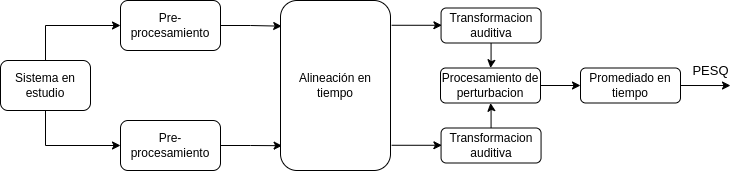
\includegraphics[scale=0.6]{images/ch4/pesq_schematic.png}}
	\caption{Diagrama en bloques de la medida PESQ. Figura tomada de \cite{speech_enhancement_theory_and_practice}.}
	\label{fig:ch4_pesq_schematic}
\end{figure}

\subsubsection{Pre-procesamiento}

La primera etapa de la PESQ tiene dos funciones. La primera es nivelar la señal de habla ruidosa y la señal procesada a un nivel estándar de audición. Las compensaciones a aplicar a cada señal se obtienen por tramos utilizando el valor RMS luego de ser filtradas por un filtro pasa-banda cuyas frecuencias de corte inferior y superior tienen un valor de 350 y 3250 Hz respectivamente.

La segunda etapa es un filtro cuya respuesta en frecuencia es similar a la respuesta en frecuencia típica de un micrófono de teléfono.

\subsubsection{Alineación}

Para poder realizar una comparación adecuada entre la señal de habla sin ruido y la señal filtrada, es necesario que éstas estén alineadas en el dominio del tiempo. Por esta razón la PESQ incorpora un proceso de alineación de ambas señales.

El proceso de alineación consta de dos pasos; primero se divide la señal en secciones de 64 ms y luego, para cada sección, se obtiene la correlación cruzada entre ambas señales. El máximo valor obtenido durante la correlación provee una estimación del retraso entre ambas señales en esa sección.

\subsubsection{Transformación auditiva}

El nivel de sonoridad percibido por el oído humano no es lineal en función de la frecuencia sino que es logarítmico, la sensación sonora de intensidad, es decir la sonoridad, se agudiza para sonidos débiles, y disminuye para sonidos fuertes. Para tener en cuenta este factor, la medida PESQ incorpora un bloque de transformación auditiva que transforma las señales en una representación de la sonoridad percibida por el oído humano.

El primer paso del bloque de transformación auditiva es obtener una estimación del espectro de potencia. La obtención se hace por medio de computar la FFT, utilizando una ventana de Hamming de 32 ms con un solapamiento del 50\%. Luego se computa el espectro basado en la escala Bark \cite{analytical_expressions_for_critical_band_rate_and_critical_bandwidth_as_a_function_of_frequency} por medio de sumar las potencias en 42 bandas.

El segundo paso del bloque de transformación auditiva es transformar el espectro de potencia a una medida de sonoridad utilizando el modelo de Zwicker \cite{a_revision_of_zwicker_s_loudness_model}.

\subsubsection{Cómputo de la perturbación}

La densidad de perturbación se obtiene como:

\begin{equation*}
	r_n(b) = S_n(b) - \bar{S}_n(b)
\end{equation*}

\noindent donde:

\begin{itemize}
	\item $S_n(b)$ es el resultado de pasar la señal original por el bloque de transformación auditiva.
	\item $\bar{S}_n(b)$ es el resultado de pasar la señal procesada por el bloque de transformación auditiva.
\end{itemize}

A la densidad de perturbación se la usa como una medida de error audible y se la utiliza para el cómputo final de la medida PESQ.

En la densidad de perturbación, para cada banda de frecuencias, habrá diferencias positivas y diferencias negativas. Una diferencia positiva, es decir $S_n(b) > \bar{S}_n(b)$, indica que un componente como el ruido se ha sumado a la señal original, mientras que una diferencia negativa, es decir $S_n(b) < \bar{S}_n(b)$, indica que un componente espectral ha sido omitido. Un componente omitido, a diferencia de un componente aditivo, no afecta en gran medida la calidad percibida, debido a los efectos de enmascaramiento. Por lo tanto, las diferencias positivas tienen más peso en el cómputo final de la PESQ que las diferencias negativas.

Una vez sopesadas las diferencias negativas y positivas se integra en frecuencia la densidad de perturbación para obtener el valor final de perturbación de cada segmento.

El valor final de la medida PESQ se obtiene promediando los valores de perturbación obtenidos para cada segmento. El rango de la medida PESQ varía entre $-0.5$ y $4.5$.

\subsection{Inteligibilidad}

Como vimos en la sección \ref{sec:intelligibility_vs_quality}, una señal de habla tiene alta inteligibilidad si los fonemas y las palabras en ella se pueden identificar correctamente.

La mayoría de las métricas de inteligibilidad se basan en la hipótesis de que ésta depende de qué tan audible sea la señal en cada banda de frecuencia. Una señal será audible en aquellas bandas de frecuencia donde la SNR es positiva. A medida que la SNR se acerque a 0 o se vuelva negativa, la señal comenzará a ser inaudible y por lo tanto la inteligibilidad tenderá a disminuir.  

El problema que tienen este tipo de métricas es que no son adecuadas para evaluar la variación de la inteligibilidad generada por filtros que utilizan ganancias variables en tiempo y frecuencia para suprimir el ruido presente en las señales de habla \cite{an_algorithm_for_intelligibility_prediction_of_time_frequency_weighted_noisy_speech}. 

En \cite{an_algorithm_for_intelligibility_prediction_of_time_frequency_weighted_noisy_speech} buscaron definir una métrica de inteligibilidad que tenga alto grado de correlación con las evaluaciones subjetivas realizadas a filtros que utilizan ganancias variables en tiempo y frecuencia. A la métrica en cuestión la nombraron Medida de inteligibilidad objetiva de corto plazo (STOI por sus siglas en inglés).

El diagrama en bloques de la STOI lo podemos ver en la figura \ref{fig:ch4_stoi_schematic}. A continuación se detalla el proceso completo para obtener la medida STOI.

\begin{figure}
	\centering
	\centerline{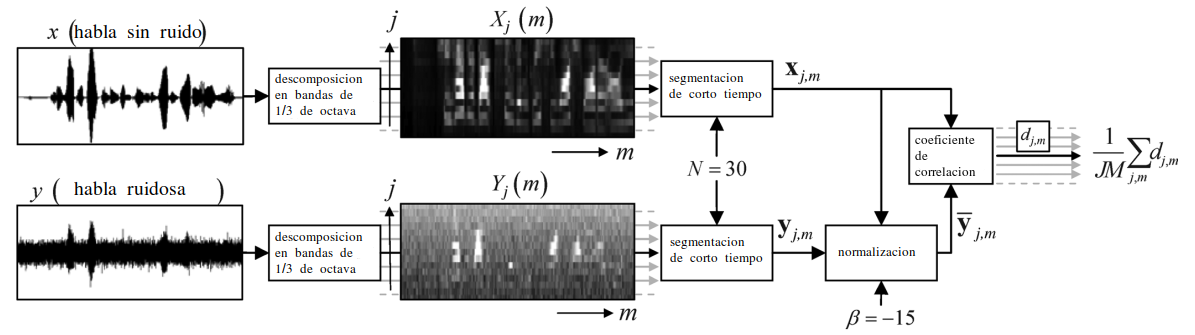
\includegraphics[scale=0.4]{images/ch4/stoi_schematic.png}}
	\caption{Diagrama en bloques de la medida STOI. Figura tomada de \cite{an_algorithm_for_intelligibility_prediction_of_time_frequency_weighted_noisy_speech}.}
	\label{fig:ch4_stoi_schematic}
\end{figure}

\subsubsection{Descomposición en bandas de 1/3 de octava}

El primer paso de la STOI es descomponer tanto la señal original como la señal procesada en tiempo y frecuencia. Para ello se aplica la STFT utilizando una ventana de Hann de 256 muestras con un solapamiento del 50\%. A cada uno de los segmentos se lo completa con 0 para que alcance un tamaño de 512 muestras.

\subsubsection{Remoción de regiones de no-habla}

El segundo paso es remover las regiones de no-habla ya que no contribuyen a la medida de inteligibilidad. Por definición la inteligibilidad depende de qué tan distinguibles sean las palabras.

Para remover las regiones de no-habla se realizan los siguientes pasos:

\begin{enumerate}
	\item Se busca la ventana con mayor energía en la señal original sin ruido.
	\item Se buscan todas las ventanas de la señal original cuyo valor de energía sea $\SI{40}{dB}$ menor al máximo encontrado en (1)
	\item Se remueven todas las ventanas encontradas en (2) tanto de la señal original como de la señal procesada
\end{enumerate}

\subsubsection{Cálculo de la unidad TF}

El tercer paso es agrupar las frecuencias en bandas de 1/3 de octava. Se usan un total de 15 bandas donde la frecuencia central de la banda más chica es 150 Hz y la de la banda más grande es de 4.3 kHz. 

La medida STOI define la unidad TF de la señal original como:

\begin{equation*}
	X_j(m) = \sqrt{\sum_{k=k_1(j)}^{k_2(j) - 1} | \hat{x}(k,m) |^2}
\end{equation*}

donde:

\begin{itemize}
	\item $j$ es el índice de la banda de 1/3 de octava
	\item $\hat{x}(k,m)$ es la muestra $k$ de la DFT de la ventana $m$ de la señal $x$
	\item $k_1$ es el límite inferior de la banda de 1/3 de octava
	\item $k_2$ es el límite superior de la banda de 1/3 de octava
\end{itemize}

La unidad TF de la señal procesada se define de igual manera y se la denota como $Y_j(m)$

Por último se definen los vectores $x_{j,m}$ y $y_{j,m}$ como:

\begin{align*}
	x_{j,m} &= [X_j(m - N + 1), X_j(m - N + 2), ..., X_j(m)]^T \\ \\
	y_{j,m} &= [Y_j(m - N + 1), Y_j(m - N + 2), ..., Y_j(m)]^T
\end{align*}

\subsubsection{Cálculo de la STOI}

La medida intermedia de inteligibilidad se calcula como el coeficiente de correlación muestral entre los vectores $x_{j,m}$ y $y_{j,m}$

\begin{equation*}
	d_{j,m} = \frac{(x_{j,m} - \mu_{x_{j,m}})^T (y_{j,m} - \mu_{y_{j,m}})}{|| x_{j,m} - \mu_{x_{j,m}} || \; ||y_{j,m} - \mu_{y_{j,m}}||}
\end{equation*}

donde $\mu_{x_{j,m}}$ es la media muestral del vector $x_{j,m}$ y $\mu_{y_{j,m}}$ es la media muestral del vector $y_{j,m}$.

Finalmente la STOI se define como

\begin{equation*}
	d = \frac{1}{JM} \sum_{j,m} d_{j,m}
\end{equation*}

donde $M$ es la cantidad total de ventanas y $J$ la cantidad de bandas de 1/3 de octava. El rango de la medida STOI varía entre $0$ y $1$

\newpage

\section{Base de datos de señales de habla y ruido}
\label{sec:audio_db}

Para poder entrenar, comparar y evaluar los algoritmos de supresión de ruido es necesario contar con una base de datos de señales de habla y otra de ruidos. Contando con ambas bases es posible generar una base de datos de señales de habla ruidosa que se utilizarán como la señal de entrada a los filtros.

A la salida de los filtros se obtendrá una señal de habla procesada o filtrada, la cual se comparará con la señal de habla sin ruido utilizando las métricas descritas en la sección \ref{sec:metrics}.

\subsection{Señales de habla}

Las señales de habla sin ruido fueron tomadas de \cite{a_scalable_noisy_speech_dataset_and_online_subjective_test_framework}, las cuales a su vez se basan en la base de datos creada en la Universidad de Edimburgo \cite{the_voice_bank_corpus}. 

La base de datos consiste en más de 20.000 oraciones leídas en voz alta por 56 oradores, 28 masculinos y 28 femeninos. Las oraciones tienen una duración media de aproximadamente 2.6 segundos y se encuentran muestreadas a 16 KHz. Las oraciones consisten, en su mayoría, en extractos del diario Scottish Herald.

\subsection{Señales de ruido}

Como vimos en \ref{sec:objetivos}, el presente trabajo se limita a estudiar el desempeño de los filtros en señales de habla corrompidas con cuatro tipos de  ruidos presentes usualmente en videoconferencias:

\begin{itemize}
	\item Tipeo: Ruido generado al escribir en un teclado.
	\item Personas hablando de fondo: Presente usualmente cuando un participante se encuentra en un ambiente público.
	\item Ruido de tráfico: Ruido presente cuando un participante se encuentra en la vía pública.
	\item Ruidos generados por mascotas: Presentes usualmente en videoconferencias domésticas. En particular se utilizaron ladridos de perro y maullidos de gato.
\end{itemize}

Las señales de ruido fueron tomadas de tres bases de datos distintas:

\begin{enumerate}
	\item La base generada por Microsoft en \cite{a_scalable_noisy_speech_dataset_and_online_subjective_test_framework}.
	\item Freesound: https://freesound.org/ .
	\item Google AudioSet: https://research.google.com/audioset/ .
\end{enumerate}

De (1) se obtuvieron señales de ruido correspondientes a la clase \emph{ruido de fondo} y \emph{tipeo}. De (2) se obtuvieron más señales correspondientes al ruido \emph{tipeo}. De (3) se obtuvieron las clases \emph{tráfico} y \emph{mascotas}.

Al igual que las señales de habla, todas las señales de ruido fueron muestreadas a 16 kHz.

\subsection{Generación de señales de habla ruidosas}
\label{sec:noisy_signals_generation}

Como dijimos al comienzo de la presente sección, a partir de la base de señales de habla y de la base de señales de ruidos, es posible generar la base de señales de habla ruidosa. 

Los algoritmos se desempeñarán de manera diferente dependiendo del nivel de ruido ($SNR$) que tenga cada una de las señales procesadas. El presente trabajo se limita a trabajar con el siguiente conjunto de niveles $SNR$:

\begin{equation*}
	\{ \SI{-5}{dB}, \; \SI{0}{dB}, \; \SI{5}{dB}, \; \SI{10}{dB}, \; \SI{15}{dB}, \; \SI{20}{dB}, \; \infty \, \si{dB} \}
\end{equation*}

El caso $SNR = \infty \, \si{dB}$ describe el caso de señales de habla sin ruido. Este caso se lo incluye porque se busca que los algoritmos no distorsionen señales que no contienen ruido.

\subsubsection{Mezcla de señales a distintos SNRs}

El primer paso para mezclar la señal de habla con la señal de ruido es normalizar ambas señales de tal manera que tengan el mismo valor RMS. A este proceso se le llama normalización RMS.

Dada una señal de habla $s[k]$ y una señal de ruido $n[k]$, supongamos que se quiere hallar $c_1$ tal que la señal $c_1 \; s[k]$ tenga cierto valor $RMS$ igual a $b$, es decir:

\begin{equation*}
	RMS\{c_1 \; s[k]\} = b
\end{equation*}

El valor RMS de la señal escalada viene dado por:

\begin{equation*}
	b = \sqrt{\frac{1}{K} \sum_{\forall k} (c_1 \; s[k])^2}
\end{equation*}

\noindent entonces:

\begin{equation*}
	c_1 = \sqrt{\frac{K \; b^2}{\sum_{\forall k} s[k]^2}} = \frac{b}{RMS\{s[k]\}}
\end{equation*}

El valor RMS escogido fue de $\SI{-25}{dB}$, entonces el factor $c$ se obtiene como:

\begin{equation*}
	c_1 = \frac{10^{\frac{-25}{20}}}{RMS\{s[k]\}}
\end{equation*}

Finalmente obtenemos:

\begin{equation*}
	s'[k] = \frac{10^{\frac{-25}{20}}}{RMS\{s[k]\}} \; s[k] \qquad \text{y} \qquad n'[k] = \frac{10^{\frac{-25}{20}}}{RMS\{s[k]\}} \; n[k]
\end{equation*}

El segundo paso es mezclar ambas señales a un determinado valor de $SNR$. Para ello debemos calcular el factor de escalado $c_2$, a aplicar en la señal de ruido, tal que:

\begin{equation*}
	SNR = \frac{RMS\{s'[k]\}}{RMS\{c_2 \; n'[k]\}}
\end{equation*}

\noindent entonces:

\begin{equation*}
	c_2 = \frac{RMS\{s'[k]\}}{SNR \quad RMS\{n'[k]\}}
\end{equation*}

\noindent y dado que usualmente el valor $SNR$ es expresado en $\si{dB}$ tenemos que:

\begin{equation*}
	c_2 = \frac{RMS\{s'[k]\}}{10^{\frac{SNR}{20}} \quad RMS\{n'[k]\}}
\end{equation*}

Luego se obtiene la señal de habla ruidosa calculando:

\begin{equation*}
	y'[k] = s'[k] + c_2 \; n'[k]
\end{equation*}

Por último es necesario contar con señales de habla ruidosas con distintas intensidades, por este motivo se realizó una nueva normalización RMS con un valor objetivo aleatorio de entre $\SI{-15}{dB}$ y $\SI{-35}{dB}$. Dado $l$ el valor RMS aleatorio en decibeles, el factor de escalado se calcula como:

\begin{equation*}
	c_3 = \frac{10^{\frac{l}{20}}}{RMS\{y[k]\}}
\end{equation*}

Finalmente la señal de habla ruidosa viene dada por:

\begin{equation*}
	y[k] = c_3 \left( s'[k] + c_2 \; n'[k] \right)
\end{equation*}

\subsubsection{Niveles base de PESQ y STOI}

Cada señal de habla ruidosa tendrá cierto nivel base para las medidas PESQ y STOI. El objetivo de los algoritmos de supresión de ruido es mejorar el nivel base.

Dependiendo de las características de cada señal ruidosa, el nivel base será diferente.

Las figuras \ref{fig:ch5_pesq_histogram} y \ref{fig:ch5_stoi_histogram} muestran un histograma de los niveles base para los distintos valores de SNR utilizados.

\begin{figure}[H]
	\centering
	\centerline{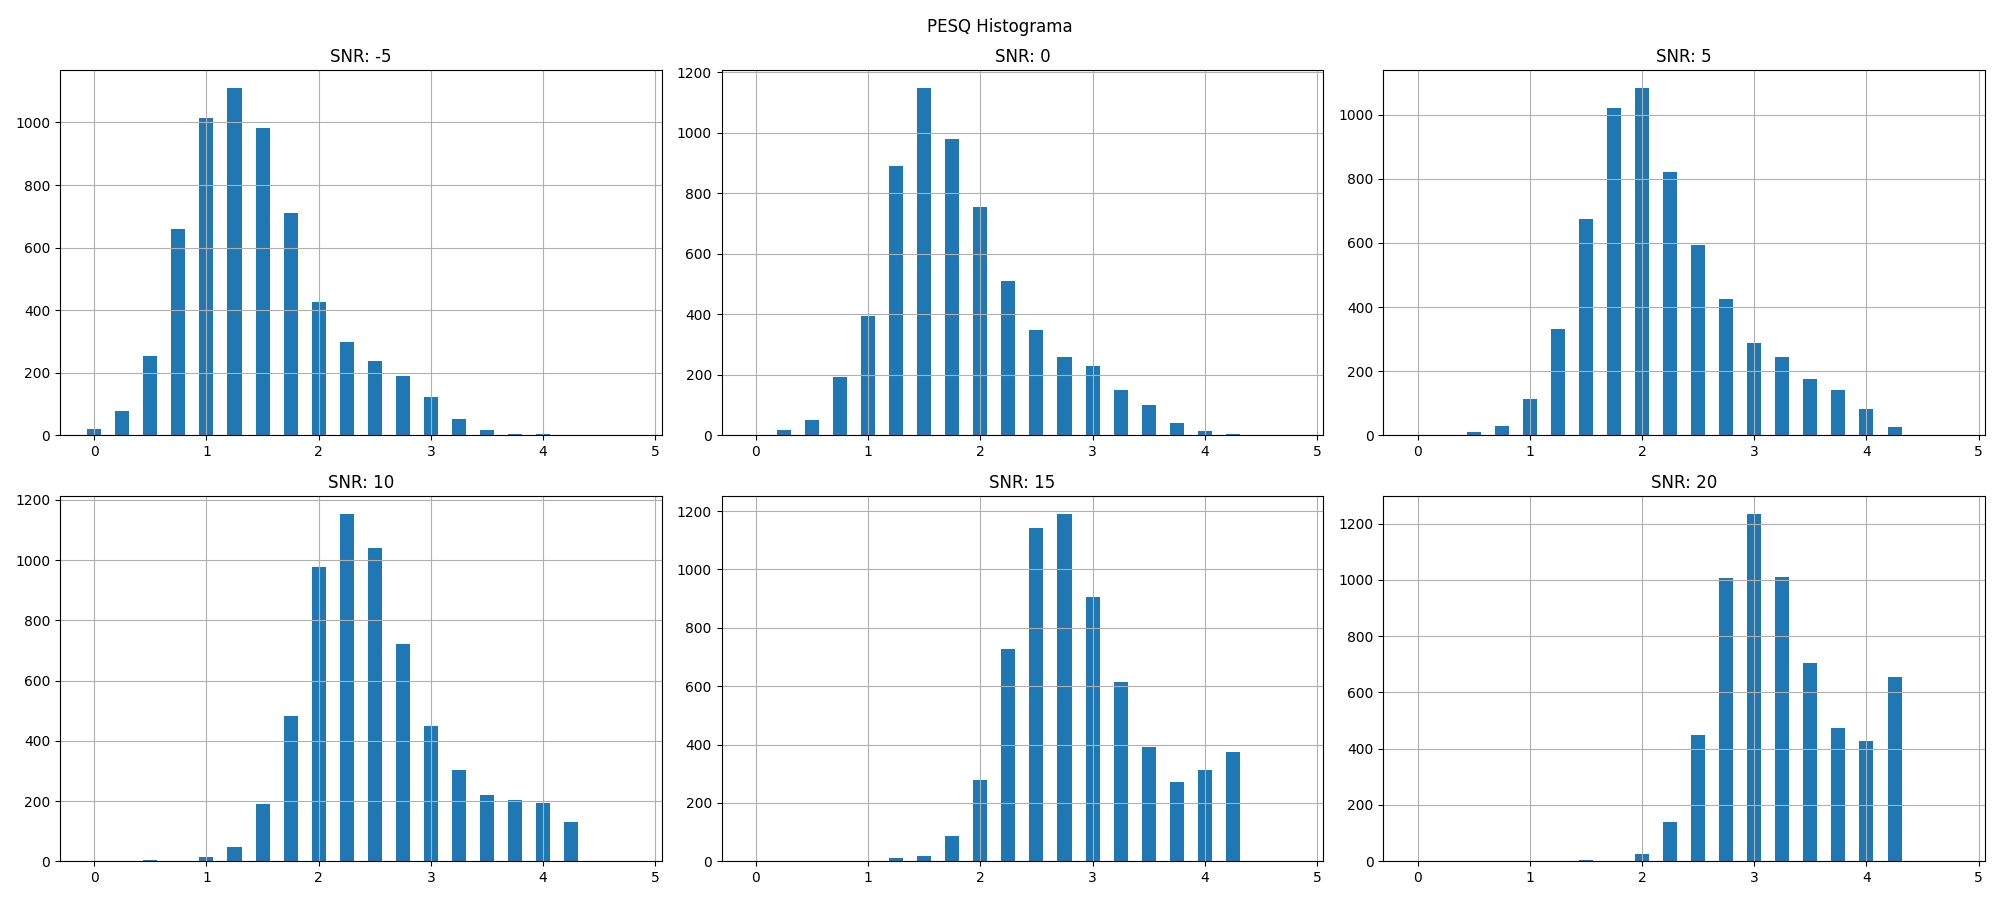
\includegraphics[scale=0.35]{images/ch5/pesq_aggregated.png}}
	\caption{Histograma PESQ.}
	\label{fig:ch5_pesq_histogram}
\end{figure}

\begin{figure}[H]
	\centering
	\centerline{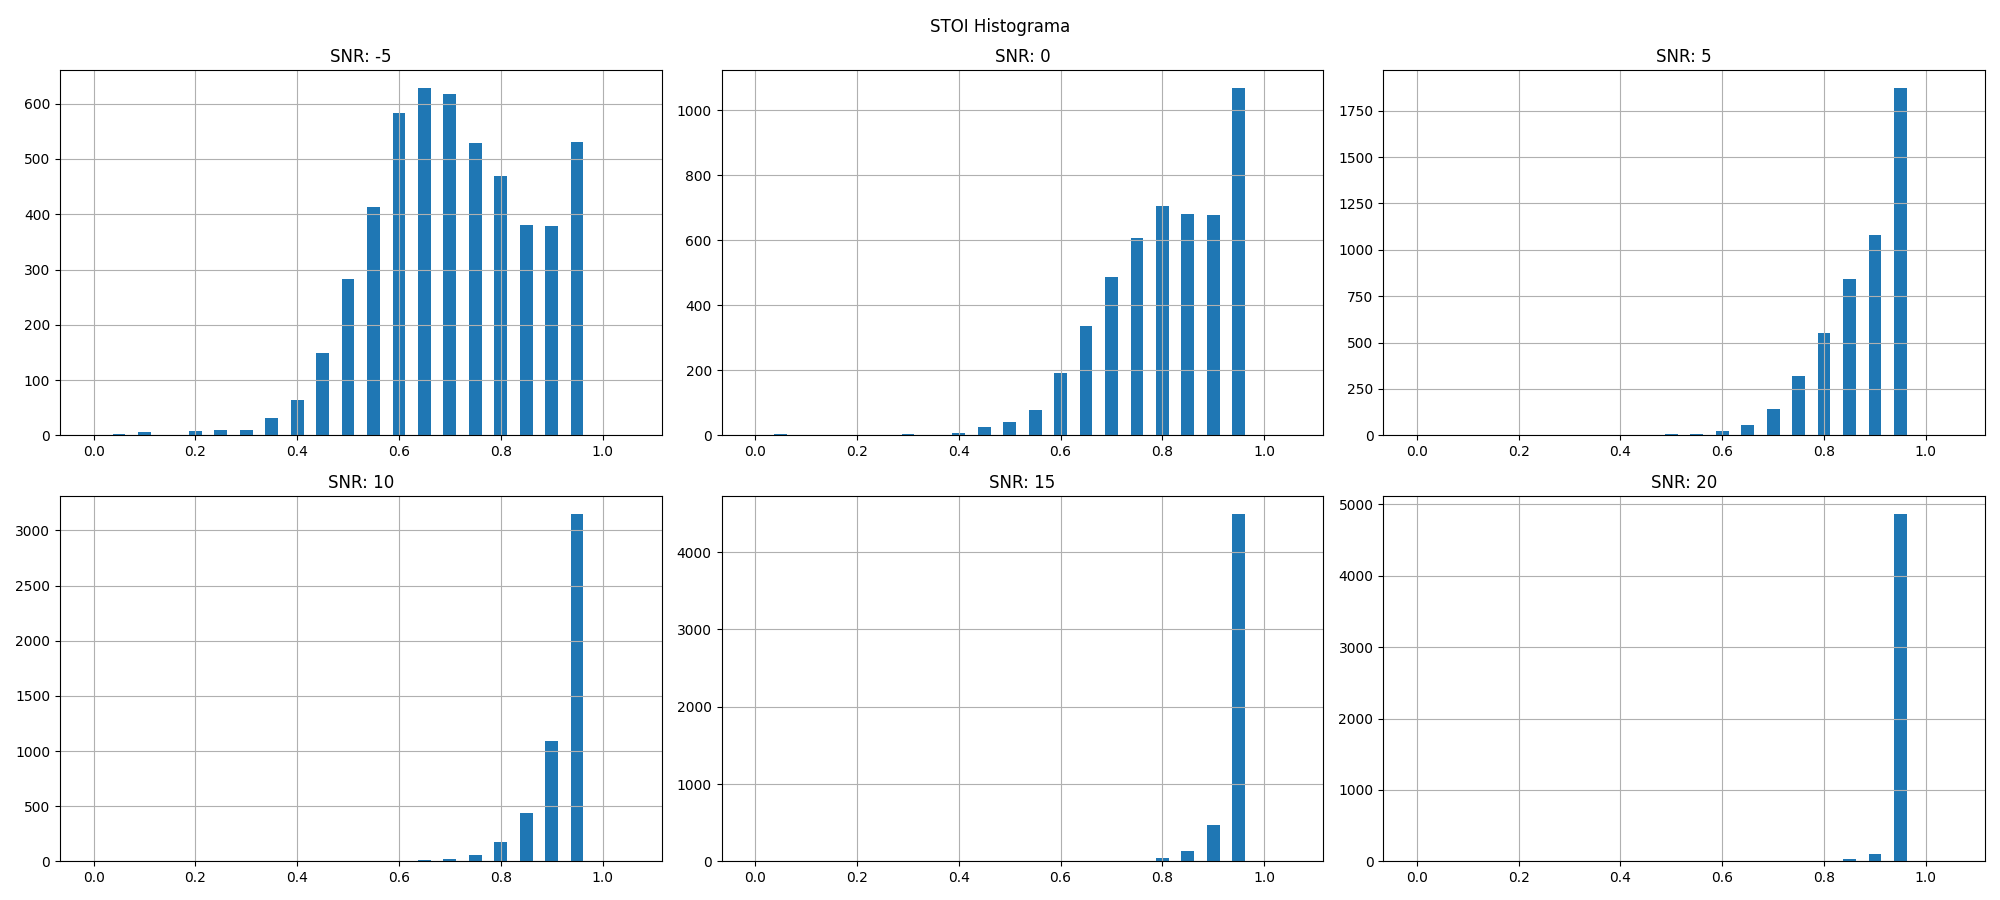
\includegraphics[scale=0.35]{images/ch5/stoi_aggregated.png}}
	\caption{Histograma STOI.}
	\label{fig:ch5_stoi_histogram}
\end{figure}

A medida que la SNR aumenta, los valores medio de PESQ y STOI se corren hacia la derecha, es decir se acercan al valor máximo, que para PESQ es de 4.5 y para STOI es de 1. Ambos límites son alcanzados cuando la SNR es infinita, es decir cuando no hay presencia de ruido en la señal de habla.

\subsection{Ruido correlacionado}

Como vimos en la sección \ref{sec:adaptive_filter_architecture}, el filtro adaptativo depende de dos señales de entrada; la señal de habla ruidosa $d(n)$ y la señal de ruido correlacionado $u(n)$. 

En la sección anterior vimos cómo se construyeron las señales de habla ruidosa mezclando señales de habla con señales de ruido, las cuales fueron obtenidas de bases de datos comúnmente utilizadas en experimentos relacionados con el presente trabajo. Sin embargo, para el caso de ruido correlacionado, no fue posible encontrar una base de datos obtenida a partir de grabaciones reales. Por tal motivo se optó por fabricar la base a partir de la base de señales de ruido.

Para fabricar el ruido correlacionado lo que se hizo fue partir la señal de ruido en bloques de largo aleatorio en el conjunto \{16384, 32768, 65536\}. Luego, a cada bloque se le aplicó un filtro $A$, nuevamente, de largo aleatorio en el rango [8, 12] cuyos coeficientes también son aleatorios en el rango [0, 1].

En una configuración como la que vimos en la figura \ref{fig:ch3_af-se-setup}, en algunas ocasiones es posible que ocurra el fenómeno de diafonía donde parte de la señal de habla $s(n)$ se mezcla con el ruido de referencia $n_2(n)$. Para simular condiciones similares a las encontradas en la práctica, además de realizar la transformación aleatoria descrita en el párrafo anterior, a la señal obtenida se le sumó un porcentaje $a$ de la señal de habla $s(n)$ aleatorio en el rango [0, 5].

Resumiendo, la señal de ruido de referencia fue obtenida como:

\begin{equation*}
	n_2(n) = A(n) \circledast n_1(n) + a(n) \cdot s(n)
\end{equation*}

\noindent donde $A(n)$ son los filtros aleatorios y $a(n)$ son los coeficientes aleatorios de diafonía.

\newpage

\section{Estado del arte}

En el presente capitulo se analizará el estado del arte de los canceladores de ruido para señales de habla captadas por un solo micrófono.

Uno de los primeros trabajos donde se estudió los canceladores de ruido con filtros basados en redes neuronales fue en; \emph{A regression approach to speech enhacement based on deep neuronal networks} \cite{a_regression_approach_to_speech_enhancement_based_on_deep_neural_networks}. Los autores del articulo son; Yong Xu, Jun Du, Li-Rong Dai, and Chin-Hui Lee y fue publicado en el año 2015.

La arquitectura de red neuronal usada es una red del tipo \emph{feedforward} completamente conectada con hasta 4 capas ocultas y cada una con hasta 2048 unidades. La base de datos usada para entrenar la red contiene 104 tipos de ruidos diferentes y un total de 100 horas de entrenamiento.

Una de las métricas usadas fue la PESQ y a continuación se detallan los valores que obtuvieron:

\begin{table}[H]
	\centering
	\begin{tabular}{ |c|c|c|c|c|c|c|c| } 
		\hline
		SNR [dB] & $-5$ & $0$ & $5$ & $10$ & $15$ & $20$ & Media \\ 
		\hline
		PESQ - Ruidosa & 1.37 & 1.61 & 1.90 & 2.22 & 2.55 & 2.88 & 2.09 \\
		PESQ - Filtrada & 1.75 & 2.09 & 2.44 & 2.78 & 3.09 & 3.37 & 2.59 \\
		STOI - Ruidosa & - & - & - & - & - & - & - \\
		STOI - Filtrada & - & - & - & - & - & - & - \\
		\hline
	\end{tabular}
	\caption{PESQ en función de la SNR.}
\end{table}

Otro de los trabajos interesantes para analizar es \emph{Speech Enhancement In Multiple-Noise Conditions using Deep Neural Networks} publicado por Anurag Kumar y Dinei Florencio en el año 2016 \cite{speech_enhancement_in_multiple_moise_conditions_using_deep_neural_networks}.

Nuevamente la arquitectura utilizada es del tipo feedforward completamente conectada con 3 unidades ocultas, cada una con 2048 unidades. La base de datos usada para entrenar la red tiene una duración total de 100 horas. 

Las medidas usadas para analizar los resultaron fueron la PESQ y la STOI. A continuación podemos encontrar los resultados que obtuvieron:

\begin{table}[H]
	\centering
	\begin{tabular}{ |c|c|c|c|c|c|c|c| } 
		\hline
		SNR [dB] & $-5$ & $0$ & $5$ & $10$ & $15$ & $20$ & Media \\ 
		\hline
		PESQ - Ruidosa & 1.46 & 1.77 & 2.11 & 2.53 & 2.88 & 3.23 & - \\
		PESQ - Filtrada & 1.92 & 2.32 & 2.69 & 3.09 & 3.40 & 3.67 & - \\
		STOI - Ruidosa & 0.612 & 0.714 & 0.813 & 0.898 & 0.945 & 0.974 & - \\
		STOI - Filtrada & 0.703 & 0.804 & 0.872 & 0.923 & 0.950 & 0.965 & - \\
		\hline
	\end{tabular}
	\caption{PESQ y STOI en función de la SNR.}
\end{table}

%Delta PESQ 0.5, 0.59, 0.63, 0.61, 0.56, 0.48
%Delta STOI 0.105, 0.098, 0.066, 0.03, 0.008, -0.004

El siguiente trabajo que resultó relevante de analizar fue uno de los primeros en proponer otro tipo de arquitectura de red neuronal. El nombre del artículo es \emph{A fully convolutional neural network for speech enhancement} publicado por Se Rim Park y Jinwon Lee en el año 2016 \cite{a_fully_convolutional_neural_network_for_speech_enhancement}. 

La arquitectura utilizada fue del tipo convolucional con 16 capas. La red contaba con un codificador y un decodificador similar a los descritos en \ref{sec:redes_autocodificadoras}. La base de datos usada para entrenar la red contiene 27 tipos de ruidos diferentes mezclados con las señales de habla únicamente a $\SI{0}{dB}$. A continuación podemos ver los resultados que obtuvieron:

\begin{table}[H]
	\centering
	\begin{tabular}{ |c|c|c|c|c|c|c|c| } 
		\hline
		SNR [dB] & $-5$ & $0$ & $5$ & $10$ & $15$ & $20$ & Media \\ 
		\hline
		PESQ - Ruidosa & - & - & - & - & - & - & - \\
		PESQ - Filtrada & - & 2.34 & - & - & - & - & - \\
		STOI - Ruidosa & - & - & - & - & - & - & - \\
		STOI - Filtrada & - & 0.83 & - & - & - & - & - \\
		\hline
	\end{tabular}
	\caption{PESQ y STOI en función de la SNR.}
\end{table}


Otro de los artículos analizados fue \emph{A Convolutional Recurrent Neural Network for Real-Time Speech} el cual utiliza una arquitectura convolucional con una capa recurrente. Ademas, lo interesante es que propone un procesamiento de las señales de manera causal para que pueda utilizarse para filtrado de ruido en tiempo real. El trabajo fue publicado por Ke Tan y DeLiang Wang en el año 2018 \cite{a_convolutional_recurrent_neural_network_for_real_time_speech_enhancement}.

La base de datos usada tiene una duración total de 126 horas y utilizan niveles de ruido en el rango [-5, 0] dB. A continuación podemos ver los resultados que obtuvieron:

\begin{table}[H]
	\centering
	\begin{tabular}{ |c|c|c|c|c|c|c|c|c| } 
		\hline
		SNR [dB] & $-5$ & $-2$ & $0$ & $5$ & $10$ & $15$ & $20$ & Media \\ 
		\hline
		PESQ - Ruidosa & 1.50 & 1.67 & - & - & - & - & - & - \\
		PESQ - Filtrada & 2.15 & 2.41 & - & - & - & - & - & - \\
		STOI - Ruidosa & 0.581 & 0.657 & - & - & - & - & - & - \\
		STOI - Filtrada & 0.778 & 0.840 & - & - & - & - & - & - \\
		\hline
	\end{tabular}
	\caption{PESQ y STOI en función de la SNR.}
\end{table}

WEIGHTED SPEECH DISTORTION LOSSES FOR
NEURAL-NETWORK-BASED REAL-TIME SPEECH ENHANCEMENT

Rango de SNRs: 0 a 40
14 tipos de ruidos
Usan una red basada en layers GRU
Usan una función de error compleja

Noisy PESQ 2.22
Noisy STOI 88

Filtered PESQ 2.65
Filtered STOI 90.7

Towards speech enhancement using a variational U-Net architecture

Rango de SNRs: 0 a 20

Cantidad de tipos de ruidos sin especificar

15 horas de entrenamiento

noisy pesq 2.52 
noisy stoi 91.51

filtered pesq 3.01 
filtered stoi 94.08

100 horas de entrenamiento

filtered pesq 3.11
filtered stoi 94.60

noisy pesq 2.52 
noisy stoi 91.51

A Perceptually-Motivated Approach for Low-Complexity, Real-Time Enhancement of Fullband Speech

Rango de SNRs: -5 a 45

Cantidad de tipos de ruidos sin especificar

120 horas de entrenamiento

filtered pesq 2.54

noisy pesq 1.97 



Feature enhancement by bidirectional LSTM networks for conversational speech recognition in highly non-stationary noise





Mi tesis 1

Rango de SNRs: -5 a 40
14 tipos de ruidos
Convolutional network

Noisy PESQ: 2.48
Filtered PESQ: 2.55

Noisy STOI: 0.89
Filtered STOI: 0.88

Mi tesis 2

Rango de SNRs: -5 a 20
14 tipos de ruidos
Convolutional network

Noisy PESQ: 2.20
Filtered PESQ: 2.40

Noisy STOI: 0.875
Filtered STOI: 0.871




\newpage

\section{Experimentación con el filtro adaptativo}

En la presente sección se describe el proceso de experimentación llevado a cabo para evaluar el rendimiento del filtro adaptativo. Para la evaluación se utilizó el conjunto de prueba de la base de datos descrita en la sección \ref{sec:audio_db}.

El proceso de pruebas consistió en ingresar al filtro adaptativo señales ruidosas, obtener la respuesta del filtro y compararla con la señal original sin ruido, por medio de las métricas STOI y PESQ.

\subsection{Parámetros del filtro}

De las ecuaciones vistas en la sección \ref{sec:filtro_adaptativo_procesamiento_de_señales} se observa que antes de poder utilizar el filtro, se necesitan definir algunos parámetros:

\begin{itemize}
	\item Cantidad de coeficientes $M$.
	\item Factor de olvido $\lambda$.
	\item Factor de regularización $\epsilon$.
\end{itemize}


A continuación veremos cómo se configuraron cada uno de ellos.

\subsubsection{Cantidad de coeficientes $M$}

El parámetro M define el largo del filtro y por ende la cantidad de coeficientes. A mayor cantidad de coeficientes mayor será la capacidad del filtro para adaptarse a los retardos entre las señales captadas por los micrófonos y también será mayor la capacidad de cancelación. Sin embargo, a medida que aumentamos la cantidad de coeficientes, también aumenta el tiempo de procesamiento. Para el presente trabajo se utilizaron 16 coeficientes, es decir $M=16$.

\subsubsection{Factor de olvido $\lambda$}

El factor de olvido $\lambda$ se debe escoger en el rango $0 \ll \lambda \le 1$. En el caso extremo de $\lambda=1$, la estimación de la matriz de autocorrelación adopta el valor

\begin{equation*}
	\hat{R}_{uu} = \frac{1}{i+1} \sum_{j=0}^{i} u_j^* u_j
\end{equation*}

\noindent es decir, se promedian todas las estimaciones anteriores de $R_{uu}$. Al elegir un valor menor a uno, se dice que se le introduce memoria a la estimación ya que se le estará dando mayor importancia a las estimaciones recientes que a las pasadas. 

El parámetro $\lambda$ define la capacidad de adaptación del algoritmo. Mientras más cerca de uno esté, más lento responderá el filtro ante cambios en las características de la señal de entrada $u$. Para el presente trabajo se encontró que una buena relación de compromiso se encuentra en el valor $\lambda=0.998$.

\subsubsection{Factor de regularización $\epsilon$}

En la sección \ref{sec:adaptive_filter_rls} vimos que, desde el punto de vista de los filtros adaptativos, el filtro RLS surge de la recursión de Newton dada por:

\begin{equation}
	w_i = w_{i-1} + \mu (\epsilon I + R_{uu} )^{-1} \left( R_{du} - R_{uu} w_{i-1} \right)
\end{equation}

El término $\epsilon I$ permite regularizar la inversión de la matriz que estima $R_{uu}$, es decir regularizar la inversa de:

\begin{equation*}
	\hat{R}_{uu} = \frac{1}{i+1} \sum_{j=0}^{i} u_j^* u_j
\end{equation*}

Desarrollando la recursión y eligiendo $\epsilon(i) = \frac{\lambda^{i+1} \epsilon }{i+1}$ se obtiene que el parámetro $\epsilon$ sólo está involucrado en la condición inicial del algoritmo. Un valor usualmente utilizado y que en el presente trabajo permitió la adecuada regularización, es el de $\epsilon=0.01$


\subsection{Resultados}

\subsubsection{Medida PESQ}

Dado el conjunto de audios de prueba con un largo igual a $P$, las señales de habla ruidosas $d_p(n)$, las señales de habla sin ruido $s_p(n)$, y las señales de habla filtradas $\hat{s}_p(n)$, se definieron las siguientes medidas.

\vspace{5mm}

\noindent $\textbf{PESQ - Ruidosa}$

\vspace{5mm}

Medida PESQ entre la señal de habla ruidosa y la señal de habla sin ruido. Establece una cota inferior en la medida PESQ que debería tener la señal de habla filtrada.

\begin{equation*}
	\textbf{PESQ - Ruidosa} = \frac{1}{P-1} \sum_{p=0}^{P-1} PESQ\{ s_p(n), d_p(n) \}
\end{equation*}

\noindent $\textbf{PESQ - Filtrada}$ 

\vspace{5mm}

Medida PESQ entre la señal de habla filtrada y la señal de habla sin ruido. 

\begin{equation*}
	\textbf{PESQ - Filtrada} = \frac{1}{P-1} \sum_{p=0}^{P-1} PESQ\{ s_p(n), \hat{s}_p(n) \}
\end{equation*}

Uno de los objetivos del filtro de ruido es mejorar, o al menos mantener, la calidad de la señal de habla, es por eso que la medida PESQ calculada para la señal ruidosa $d(n)$ nos da una cota inferior, es decir se espera que:

\begin{equation*}
	\text{PESQ - Filtrada} \geq \text{PESQ - Ruidosa}
\end{equation*}

Como vimos en la sección \ref{sec:metrics}, las señales de habla ruidosa fueron construidas utilizando distintos valores de SNR. Una forma de evaluar el filtro es analizar qué tanto cambia la PESQ para cada valor de SNR utilizado.

En la figura \ref{fig:ch6_pesq_by_snr} podemos ver las medidas \textbf{PESQ - Ruidosa} y \textbf{PESQ - Filtrada} en función del nivel de ruido. En la gráfica se observa que una vez superado los $\SI{5}{dB}$, el filtro empeoró la calidad de las señales de audio.

\begin{figure}
	\centering
	\centerline{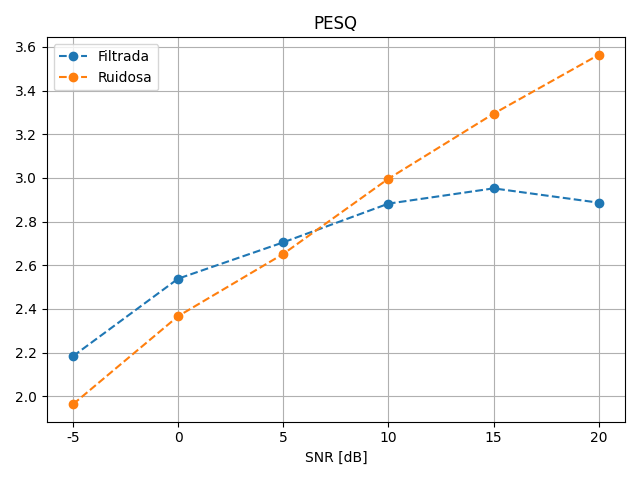
\includegraphics[scale=0.75]{images/ch6/pesq_by_snr.png}}
	\caption{PESQ en función de la SNR.}
	\label{fig:ch6_pesq_by_snr}
\end{figure}

A medida que la SNR fue aumentando, le resultó cada vez más difícil al filtro poder mejorar el valor de base de la medida $PESQ$. En la siguiente sección se analiza este comportamiento mas en detalle. En la tabla \ref{table:pesq_by_snr} podemos ver el detalle de los resultados de la figura \ref{fig:ch6_pesq_by_snr}.

\begin{table}
	\centering
	\begin{tabular}{ |c|c|c|c|c|c|c| } 
		\hline
		SNR [dB] & $-5$ & $0$ & $5$ & $10$ & $15$ & $20$ \\ 
		\hline
		PESQ - Ruidosa & 1.96 & 2.36 & 2.65 & 2.99 & 3.29 & 3.56 \\
		PESQ - Filtrada & 2.18 & 2.54 & 2.70 & 2.89 & 2.95 & 2.89 \\
		\hline
	\end{tabular}
	\caption{PESQ en función de la SNR.}
	\label{table:pesq_by_snr}
\end{table}

% [2199] Noisy PESQ: 2.799255890755177
% [2199] Filtered PESQ: 2.6858125135325936
% [2199] Noisy STOI: 0.9270031623427075
% [2199] Filtered STOI: 0.9450888375748907~

Otra forma de evaluar el filtro es analizar cómo varían las medidas en función del tipo de ruido. En la figura \ref{fig:ch6_pesq_by_noise_type} podemos ver la medida PESQ en función del tipo de ruido.

\begin{figure}
	\centering
	\centerline{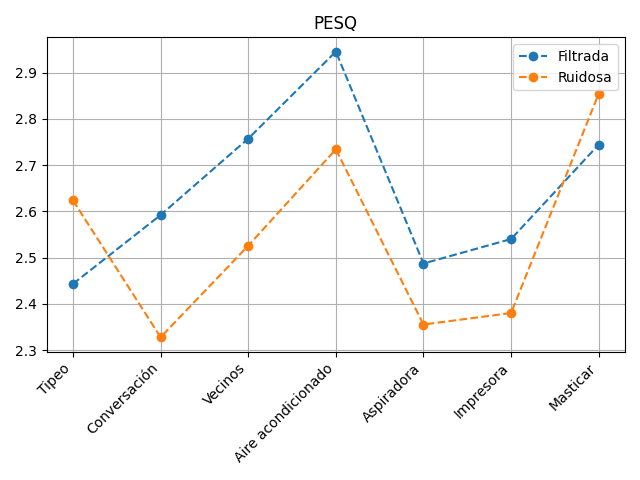
\includegraphics[scale=0.75]{images/ch6/pesq_by_noise_type.png}}
	\caption{PESQ en función del tipo de ruido.}
	\label{fig:ch6_pesq_by_noise_type}
\end{figure} 

% [2199] Noisy PESQ: 2.9368886407946886
% [2199] Filtered PESQ: 2.8188107138075527
% [2199] Noisy STOI: 0.9390761638343121
% [2199] Filtered STOI: 0.9533274579765317

El filtro adaptativo logró mejorar la calidad de las señales ruidosas en los tipos de ruidos; \emph{Conversación}, \emph{Vecinos}, \emph{Aire acondicionado}, \emph{Aspiradora} e \emph{Impresora}. Para los ruidos del tipo \emph{Tipeo} y \emph{Masticar}, la calidad disminuyó. Estos ruidos tienen la característica de ser de corta duración, lo que representa un inconveniente para el filtro adaptativo que necesita cierto tiempo para adaptarse a las nuevas condiciones de ruido y filtrarlo.

\subsubsection{Medida STOI}

Al igual que para la PESQ se analizaron las siguientes medidas.

\vspace{5mm}

\noindent $\textbf{STOI - Ruidosa}$

\vspace{5mm}

Medida STOI entre la señal de habla ruidosa y la señal de habla sin ruido. Establece una cota inferior en la medida STOI que debería tener la señal de habla filtrada.

\begin{equation*}
	\textbf{STOI - Ruidosa} = \frac{1}{P-1} \sum_{p=0}^{P-1} STOI\{ s_p(n), d_p(n) \}
\end{equation*}

\noindent $\textbf{STOI - Filtrada}$ 

\vspace{5mm}

Medida STOI entre la señal de habla filtrada y la señal de habla sin ruido. 

\begin{equation*}
	\textbf{STOI - Filtrada} = \frac{1}{P-1} \sum_{p=0}^{P-1} STOI\{ s_p(n), \hat{s}_p(n) \}
\end{equation*}

En la figura \ref{fig:ch6_stoi_by_snr} podemos ver las medidas \textbf{STOI - Ruidosa} y \textbf{STOI - Filtrada} en función del nivel de ruido. Al igual que para la PESQ, a partir de los $\SI{10}{dB}$ el filtro en lugar de mejorar la inteligibilidad, la empeora.  En la tabla \ref{table:stoi_by_snr} podemos ver el detalle de los resultados de la figura \ref{fig:ch6_stoi_by_snr}.

\begin{figure}
	\centering
	\centerline{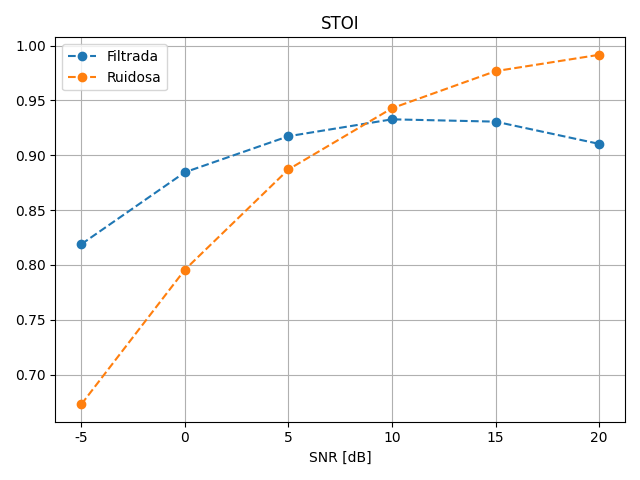
\includegraphics[scale=0.75]{images/ch6/stoi_by_snr.png}}
	\caption{STOI en función de la SNR.}
	\label{fig:ch6_stoi_by_snr}
\end{figure}

\begin{table}[ht]
	\centering
	\begin{tabular}{ |c|c|c|c|c|c|c| } 
		\hline
		SNR [dB] & $-5$ & $0$ & $5$ & $10$ & $15$ & $20$ \\ 
		\hline
		STOI - Ruidosa & 0.80 & 0.89 & 0.93 & 0.97 & 0.98 & 0.99 \\
		STOI - Filtrada & 0.89 & 0.94 & 0.95 & 0.97 & 0.97 & 0.96 \\
		\hline
	\end{tabular}
	\caption{STOI en función de la SNR.}
	\label{table:stoi_by_snr}
\end{table}

También se analizó la medida STOI como función del tipo de ruido. En la figura \ref{fig:ch6_stoi_by_noise_type} podemos ver dicha gráfica. Se observa la misma tendencia que para la medida PESQ, es decir, el desempeño en los ruidos \emph{Conversación}, \emph{Vecinos}, \emph{Aire acondicionado}, \emph{Aspiradora} y \emph{Impresora} fue mejor que en \emph{Tipeo} y \emph{Masticar}.

\begin{figure}
	\centering
	\centerline{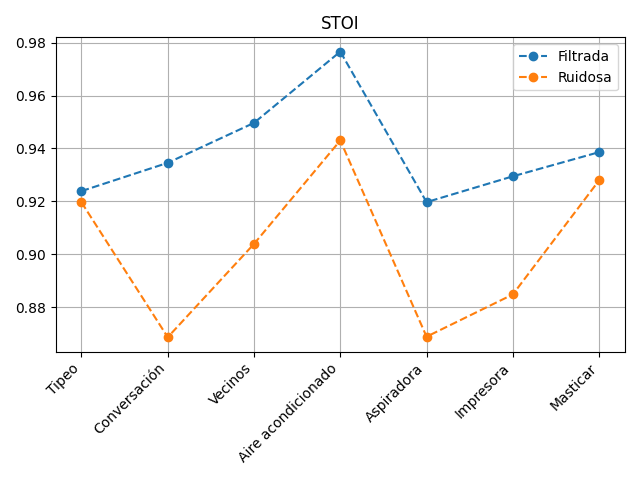
\includegraphics[scale=0.75]{images/ch6/stoi_by_noise_type.png}}
	\caption{STOI en función del tipo de ruido.}
	\label{fig:ch6_stoi_by_noise_type}
\end{figure} 

\subsubsection{Error cuadrático medio y nivel de ruido}

Dada las señales de habla sin ruido $s_p(n)$, las señales filtrada $\hat{s}_p(n)$, las señales de ruido $n_p(n)$, $N_p$ el largo de la señal $p$ y $P$ la cantidad de señales de audio en la base de datos de pruebas, se computa el error cuadrático medio, para cada uno de los niveles de ruido, como:

\begin{equation*}
	\text{ECM} = \frac{1}{P-1} \sum_{p=0}^{P} \frac{1}{N_p-1} \sum_{n=0}^{N_p} (\hat{s}_p(n) - s_p(n))^2
\end{equation*}

También definimos el nivel de ruido medio al cuadrado como:

\begin{equation*}
	\text{Nivel de ruido} = \frac{1}{P-1} \sum_{p=0}^{P} \frac{1}{N_p-1} \sum_{j=0}^{N_p} (n_p(n))^2
\end{equation*}

\begin{figure}
	\centering
	\centerline{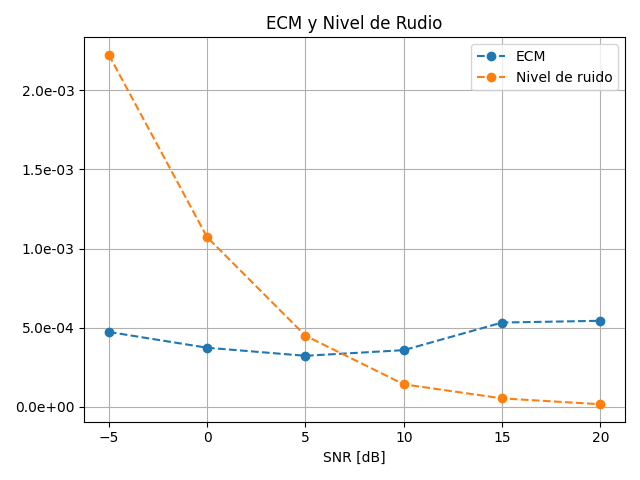
\includegraphics[scale=0.8]{images/ch6/ecm_and_noise_level.png}}
	\caption{ECM y Nivel de ruido.}
	\label{fig:ch6_mse_and_noise_level}
\end{figure}

En la figura \ref{fig:ch6_mse_and_noise_level} podemos el error cuadrático medio y el nivel de ruido como función de la SNR. En las figuras \ref{fig:ch6_pesq_by_snr} y \ref{fig:ch6_stoi_by_snr} vimos que a medida que la SNR aumentó, al filtro le resultó cada vez más difícil lograr una mejora en las medidas PESQ y STOI. 

Una explicación a este comportamiento lo podemos ver en la figura \ref{fig:ch6_mse_and_noise_level}, donde observamos que a medida que la SNR aumenta, el error cuadrático medio se vuelve comparable con el nivel ruido. Esto lleva a que las medidas  \textbf{PESQ - Filtrada} y \textbf{STOI - Filtrada} sean similares o menores que lo niveles base \textbf{PESQ - Ruidosa} y \textbf{STOI - Ruidosa}, respectivamente. En estos casos, la señal de habla filtrada tiene un nivel de ruido similar a la señal de habla ruidosa original, pero esta vez inducido por el error en estado estacionario del filtro adaptativo \cite{fundamentals_of_adaptive_filtering}.

\subsubsection{Variación de los coeficientes en función del tiempo}

Es interesante ver cómo se comportan los coeficientes del filtro para algunos ejemplos concretos. En la figura \ref{fig:ch6_variacion_temporal_de_coeficientes}  podemos ver la variación de los coeficientes del filtro en función del tiempo para 4 audios distintos. 

\begin{figure}
	\centering
	\centerline{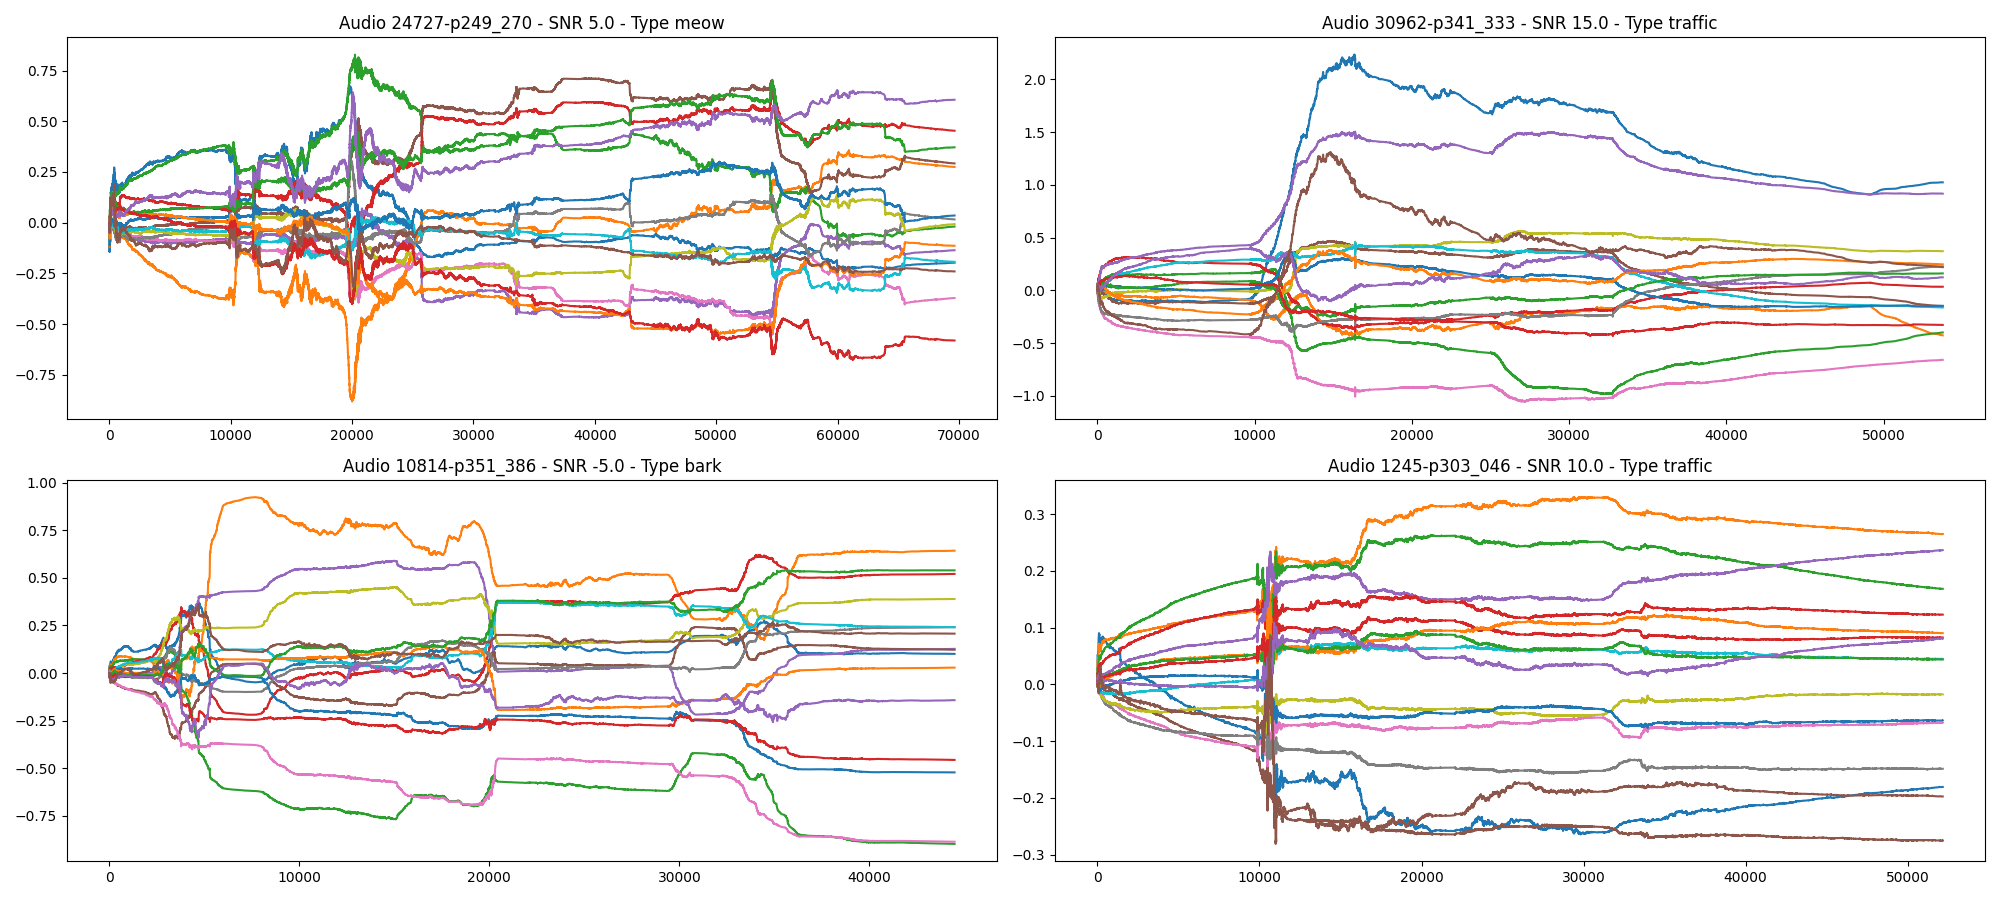
\includegraphics[scale=0.35]{images/ch6/weights.png}}
	\caption{Variación de los coeficientes en función del tiempo.}
	\label{fig:ch6_variacion_temporal_de_coeficientes}
\end{figure}

Se observa como los coeficientes se adaptan a medida que cambia la correlación entre los ruidos $n_1(n)$ y $n_2(n)$. Una vez que encuentran la nueva adaptación que minimiza el error, permanecen en un estado estacionario hasta que ocurre un nuevo cambio en el entorno.

\newpage

\section{Experimentación con el filtro neuronal}

A diferencia del filtro adaptativo, el filtro neuronal necesita una etapa de entrenamiento, con lo que la experimentación se llevó a cabo en dos etapas, la primera de entrenamiento y la segunda de evaluación. 

Nuevamente, antes de poder utilizar el filtro neuronal es necesario realizar una calibración de sus parámetros.

\subsection{Parámetros del filtro}

De las ecuaciones vistas en la sección \ref{sec:tecnicas_filtrado_redes_neuronales} se desprende que es necesario definir los siguientes parámetros:

\begin{itemize}
	\item \textbf{L} Tamaño de la ventana en la STFT.
	\item \textbf{N} Tamaño de la DFT usada para computar la STFT o cantidad de muestras en el dominio de la frecuencia en la STFT.
	\item \textbf{R} Solapamiento de ventanas o tasa de muestreo en el tiempo en la STFT.
	\item \textbf{J} Cantidad de ventanas que conforman la STFT o cantidad de muestras en el dominio del tiempo en la STFT. 
	\item Función de error.
	\item Algoritmo de entrenamiento.
	\item Tamaño de los lotes de entrenamiento.
	\item Estructura de la red neuronal.
\end{itemize}

\subsubsection{L Tamaño de la ventana en la STFT}

El tamaño de la ventana en la STFT afecta distintas características del filtrado:

\begin{itemize}
	\item Relación de compromiso entre la resolución en el dominio de la frecuencia y la resolución en el dominio del tiempo. Recordemos de la sección \ref{sec:espectrograma}, que es preferible tener más resolución en tiempo para poder reconocer los distintos sonidos. Por ende mientras más chica sea el tamaño de la ventana mejor.
	\item La señal de audio filtrada se obtiene de a una ventana a la vez, por lo tanto también es preferible una ventana corta para así tener el menor retraso posible.
	\item A medida que la ventana se hace mas chica, a un mismo poder de cómputo, aumenta el tiempo de procesamiento, ya que se necesitan más pasadas por la red neuronal.
\end{itemize}

Como se observa en la descripción anterior, no hay una forma analítica o directa de establecer el tamaño de la ventana. Un valor que se encontró experimentalmente y que mantiene una relación de compromiso adecuada entre los efectos antes mencionados, es de $\SI{16}{ms}$ o $\SI{32}{ms}$. En el presente trabajo se escogió $\SI{16}{ms}$.

Dado que las señales se encuentran muestreadas a $16 Khz$, esto nos da un largo de ventana igual a:

\begin{equation*}
	L = \SI{16}{ms} \cdot \SI{16}{KHz} = 256
\end{equation*}

\subsubsection{N Cantidad de muestras en el dominio de la frecuencia en la STFT}
\label{sec:cantidad_muestras_frecuencia}

La tasa de muestreo en frecuencia afecta las siguientes características:

\begin{itemize}
	\item A medida que aumentamos la tasa de muestreo en frecuencia, mayor resolución tendremos en ella.
	\item A medida que aumentamos la resolución en frecuencia aumenta el tiempo de cómputo de la FFT y aumenta la cantidad de parámetros de las capas convolucionales de la red neuronal.
	\item Recordemos de la sección \ref{sec:muestreo_en_tiempo_y_frecuencia} que $R \leq L \leq N$, es decir $N \ge 256$.
\end{itemize}

Nuevamente tenemos una relación de compromiso que debemos mantener en el nivel adecuado. Para el presente trabajo se utilizó una FFT de $2^{9} = 512$ puntos. 

\subsubsection{R Solapamiento de ventanas en la STFT}

En la sección \ref{sec:overlapp_and_and} vimos que una elección que permite recuperar la señal de entrada dada la STFT, es utilizar una ventana de Hamming que cumpla la relación $R = L/2$. Dado que en nuestro caso tenemos $L = 256$, obtenemos que $R=128$. Con este valor de $R$ también verificamos la condición necesaria $R \leq L \leq N$, ya que tenemos $128 \leq 256 \leq 512$.

\subsubsection{J Cantidad de muestras en el dominio del tiempo en la STFT}
\label{sec:ventanas_en_espectrogramas}

La cantidad de ventanas a incluir en cada espectrograma, define qué tanta información hacia atrás en el tiempo puede ver la red neuronal, para predecir la ventana de señal de habla filtrada en el tiempo i. 

Al aumentar o disminuir la cantidad de ventanas $J$ tendremos que:

\begin{itemize}
	\item A mayor cantidad de ventanas, más información tendrá la red para predecir y por ende menor el error de predicción. También, más grande es la dimensión del espectrograma y por ende mayor será la cantidad de parámetros de las capas convolucionales de la red neuronal.
	\item A partir de cierto punto difuso no tiene sentido seguir aumentando la cantidad de ventanas, ya que la ventana en el tiempo $i$ deja de estar correlacionada con la ventana $i - J - 1$ y por ende, no hay información útil que la red pueda utilizar en la predicción de la ventana $i$.
\end{itemize}

Experimentalmente se encontró que un número razonable de ventanas es $J=64$.

\subsubsection{Función de error o función de costo}

La función de error define la medida que se busca minimizar durante el entrenamiento de la red. El objetivo de esta función es, permitir ajustar los pesos de la red de tal manera que la medida sea cada vez más chica. En nuestro caso, a la salida de la red tenemos una ventana de la señal filtrada en el dominio de la frecuencia y como valor objetivo tenemos una ventana de la señal de habla sin ruido, también en el dominio de la frecuencia. La función de costo calcula el error entre lo obtenido a la salida de la red y el valor objetivo. 

La función de costo más adecuada para la tarea en cuestión es el error cuadrático medio:

\begin{equation*}
	l = \frac{1}{K} \sum_{i=1}^K (Y(n_i, w_i) - X(n_i, w_i))^2
\end{equation*}

\subsubsection{Algoritmo de entrenamiento}

Para poder entrenar la red neuronal es necesario escoger un optimizador. Los optimizadores se pueden ver como funciones que definen la metodología en la que se van a actualizar los pesos de la red. En el caso de los filtros adaptativos, los distintos tipos de optimizadores utilizados dan lugar a distintos filtros como el LMS, el NLMS, el RLS, etc.

Dos algoritmos, comúnmente utilizados para entrenar redes neuronales, son el método de gradiente estocástico con momento \cite{deep_learning} y el método Adam \cite{adam_optimizer}. Usualmente, el método Adam converge mas rápido gracias al uso de momentos de segundo orden.

Configurar correctamente los hiper-parámetros del optimizador resulta esencial para poder minimizar, tanto el error durante el entrenamiento como el error de generalización.

Para escoger el optimizador adecuado se evaluaron ambos experimentalmente y con Adam se obtuvieron mejores resultados, con respecto al error de generalización y la velocidad de entrenamiento. 

El optimizador Adam depende de tres hiper-parámetros, $\eta$, $\beta_1$ y $\beta_2$. El parámetro $\eta$ define la tasa de aprendizaje y los parámetros $\beta_1$ y $\beta_2$ permiten ajustar las estimaciones del valor medio y la varianza del gradiente de la función de error. Para el presente trabajo los valores utilizados fueron: $lr=1e^{-4}$, $\beta_1=0.9$ y $\beta_2=0.999$.

\subsubsection{Tamaño de los lotes de entrenamiento}

El tamaño de lote de entrenamiento define cuántas muestras deben pasar por la red, antes de calcular el error y ajustar los pesos o parámetros. El rango en el que debe estar el tamaño de lote es entre una muestra y el tamaño del conjunto de entrenamiento completo. En general, en lo referido al entrenamiento de redes neuronales, se suele utilizar el concepto de \emph{mini-batch}, es decir un lote pequeño. 

Idealmente, el tamaño del lote debería ser el conjunto de entrenamiento completo pero esto trae varios problemas.

\begin{itemize}
	\item Se ha demostrado experimentalmente que tamaños de lotes grandes afectan negativamente el error de generalización de la red \cite{on_large_batch_training}.
	\item Un lote grande requiere mucha memoria, la cual suele ser limitada en especial cuando el entrenamiento se lo realiza en una o mas GPUs.
\end{itemize}

Por otro lado, si el tamaño de lote es muy pequeño, el algoritmo de optimización no logra encontrar la dirección de minimización. En estos casos, el gradiente presenta una gran variación muestra a muestra.

Por último, en nuestro caso, debemos también tener en cuenta que una señal de habla no es la muestra que ingresa a la red sino que lo que ingresa a la red son espectrogramas de esa señal de habla. Las señales de habla utilizadas en el presente trabajo tienen en promedio 80 espectrogramas. Es esencial para el entrenamiento adecuado de la red, que antes de cada actualización de los parámetros se haya pasado por la red muestras de distintos audios, de lo contrario el optimizador no logrará encontrar la dirección de minimización. En el presente trabajo, durante el entrenamiento, se utilizó un tamaño de lote de $500$ muestras.

\subsubsection{Estructura de la red neuronal}

En la sección \ref{sec:cantidad_muestras_frecuencia} vimos que el largo de la DFT utilizada para el cómputo de la STFT es de $N=512$. Las señales de habla son señales reales, con lo cual la DFT tendrá simetría conjugada, esto nos lleva a que la información espectral esté duplicada.

Utilizar toda la DFT es innecesario e implicaría un tiempo de cómputo mayor. Debido a la simetría que presenta, toda la información útil de la DFT la podemos encontrar en cada una de las mitades de la simetría. Esto nos lleva a que los espectrogramas que sirven como entrada a la red están conformados por $256$ muestras en el dominio de la frecuencia.

Por otro lado, en la sección \ref{sec:ventanas_en_espectrogramas}, vimos que la cantidad de ventanas a incluir en un espectrograma es de $J=64$. Esto nos lleva a obtener el tamaño de los espectrogramas, el cual es de $256 \times 64$. El tamaño de los espectrogramas resulta esencial para definir la estructura de la red.

Como vimos en la sección \ref{sec:redes_tipo_u}, a medida que los espectrogramas pasan por las distintas capas de la red, el tamaño se irá reduciendo hasta terminar el camino del codificador. Luego, pasan a la parte del decodificador, donde el tamaño se va recuperando capa a capa. En el codificador, a medida que se reduce el tamaño se aumenta la cantidad de filtros presentes en la capa convolucional. En el decodificador, a medida que se aumenta el tamaño, se reduce la cantidad de filtros.

En la figura \ref{fig:ch7_red_estructura} podemos ver cómo se va modificando el tamaño de los espectrogramas a medida que pasan por las distintas capas de la red. La notación es \textbf{Tamaño en frecuencia} $\times$ \textbf{Tamaño en tiempo} $\times$ \textbf{Canales}. Cada canal representa el resultado de la convolución entre la entrada y uno de los filtros de la capa.

\begin{figure}
	\centering
	\centerline{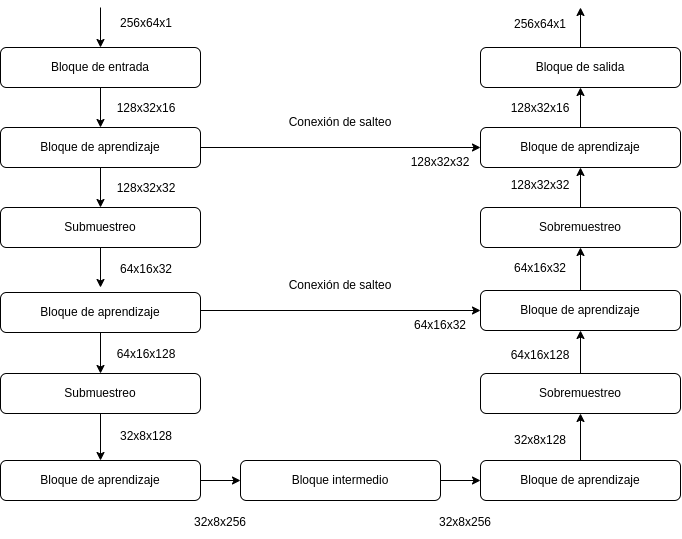
\includegraphics[scale=0.65]{images/ch7/red_estructura.png}}
	\caption{Estructura del filtro neuronal.}
	\label{fig:ch7_red_estructura}
\end{figure}

\subsection{Entrenamiento}

El entrenamiento de la red consiste en pasar por ella espectrogramas de señales ruidosas, obtener el error respecto de los espectrogramas de las señales sin ruido y modificar los pesos de la red de acuerdo a ese error.

Usualmente, durante el entrenamiento, se le muestra a la red más de una vez cada muestra del conjunto de entrenamiento. Es posible que después de cierto punto, la red empiece a aprenderse por fuerza bruta el conjunto de entrenamiento con lo que el error de generalización comienza a aumentar. Para poder detectar este momento se suele introducir una etapa de validación cada x lotes de entrenamiento, la cual es realizada contra el conjunto de prueba. 

La validación se ejecutó cada 1.000 lotes de entrenamiento y en cada una se utilizó un total de 500 audios elegidos de manera aleatoria del conjunto de prueba. En la etapa de validación del lote 40.000 se observó que el error de generalización aumentó y el aumento fue confirmado en los siguientes lotes, por lo que el entrenamiento fue detenido. Dado que a partir del lote 40.000, el error comenzó a aumentar, el modelo seleccionado fue el obtenido en dicho lote y se descartaron los siguientes. En la figura \ref{fig:ch7_entrenamiento_mse} podemos ver el error cuadrático medio durante el entrenamiento.

\begin{figure}
	\centering
	\centerline{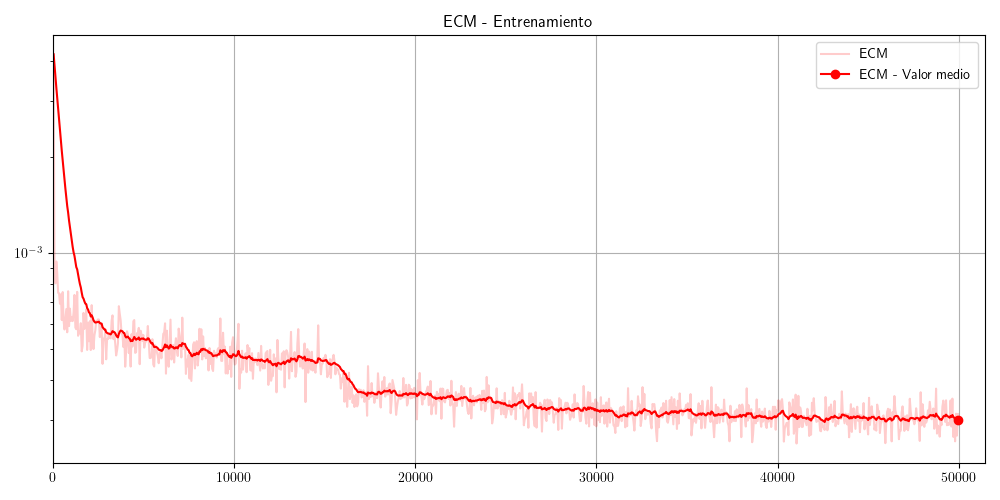
\includegraphics[scale=0.65]{images/ch7/train_mse.png}}
	\caption{Error cuadrático medio durante el entrenamiento.}
	\label{fig:ch7_entrenamiento_mse}
\end{figure}

\subsection{Resultados}
\label{sec:resultados_filtro_neuronal}

\subsubsection{Medida PESQ}

Al igual que para el caso del filtro adaptativo, se puso a prueba el desempeño del filtro neuronal en el conjunto de pruebas, computando las mismas medidas PESQ para cada uno de los niveles de ruido utilizados. 

En la figura \ref{fig:ch7_pesq_by_snr} podemos ver las medidas \textbf{PESQ - Ruidosa} y \textbf{PESQ - Filtrada} en función del nivel de ruido. Se observa que la máxima mejora media en PESQ se logra para los $\SI{5}{dB}$. Para SNRs menores y mayores, la mejora media en la PESQ disminuye manteniéndose positiva. En la tabla \ref{table:ch7_pesq_by_snr} podemos ver el detalle de los resultados de la figura \ref{fig:ch7_pesq_by_snr}.

\begin{figure}
	\centering
	\centerline{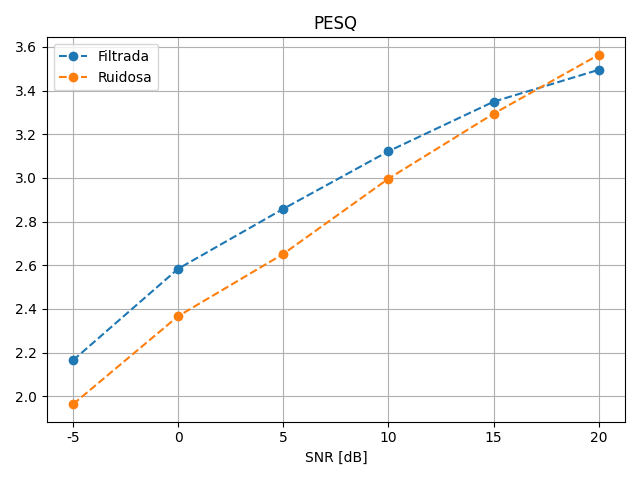
\includegraphics[scale=0.75]{images/ch7/pesq_by_snr.png}}
	\caption{PESQ en función de la SNR.}
	\label{fig:ch7_pesq_by_snr}
\end{figure}

\begin{table}
	\centering
	\begin{tabular}{ |c|c|c|c|c|c|c|c| } 
		\hline
		SNR [dB] & $-5$ & $0$ & $5$ & $10$ & $15$ & $20$ & Media \\ 
		\hline
		PESQ - Ruidosa & 1.22 & 1.59 & 1.99 & 2.42 & 2.83 & 3.20 & 2.20 \\
		PESQ - Filtrada & 1.38 & 1.86 & 2.31 & 2.68 & 2.96 & 3.23 & 2.40 \\
		\hline
	\end{tabular}
	\caption{PESQ en función de la SNR.}
	\label{table:ch7_pesq_by_snr}
\end{table}

En la figura \ref{fig:ch7_pesq_by_noise_type} podemos ver la medida PESQ en función del tipo de ruido. Se observa que para todas las clases de ruido, el filtro neuronal, en promedio, logró mejorar la calidad de las señales ruidosas. Este comportamiento va en linea con lo observado en la figura \ref{fig:ch7_pesq_by_snr} donde vimos que para todos los niveles de ruido, se logró una mejora en la calidad. 

Las clases de ruido donde el filtro logró el mejor desempeño fue en; \emph{Aire Acondicionado}, \emph{Aspiradora} e \emph{Impresora}. Esto se debe a que estas clases de ruido son mas estacionarias y por ende le es mas fácil a la red neuronal poder caracterizarlas.

\begin{figure}
	\centering
	\centerline{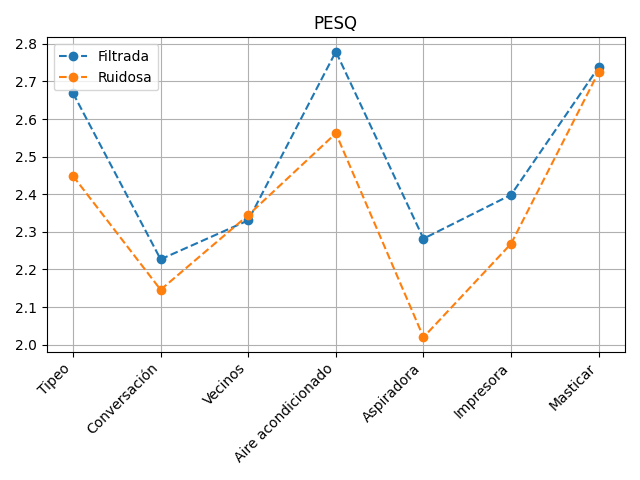
\includegraphics[scale=0.75]{images/ch7/pesq_by_noise_type.png}}
	\caption{PESQ en función del tipo de ruido.}
	\label{fig:ch7_pesq_by_noise_type}
\end{figure} 

En el ruido \emph{Vecinos} y \emph{Conversación} hay personas hablando, cuyas voces se mezclan con la señal de habla principal, dificultándole a la red identificar cuál es la señal a filtrar.

El tipo de ruido \emph{Masticar} y el tipo de ruido \emph{Tipeo} resultan ser el mas complejo de filtrar y se debe a que es altamente no-estacionario y de corta duración dificultándole a la red caracterizarlo adecuadamente. 

\subsubsection{Medida STOI}

Se puso a prueba el desempeño del filtro neuronal en el conjunto de pruebas, computando las medidas STOI ya definidas, para cada uno de los niveles snr y tipos de ruidos utilizados. 

En la figura \ref{fig:ch7_stoi_by_snr} podemos ver las medidas \textbf{STOI - Ruidosa} y \textbf{STOI - Filtrada} en función del nivel de ruido. Se observa que la máxima mejora media en STOI se logra para los $\SI{-5}{dB}$, y para SNRs mayores, la mejora media en la STOI disminuye. A partir de los $\SI{5}{dB}$ la señal filtrada tiene menor STOI que la señal ruidosa original. En el cuadro \ref{table:ch7_stoi_by_snr} podemos ver el detalle de los resultados de la figura \ref{fig:ch7_stoi_by_snr}.

\begin{figure}
	\centering
	\centerline{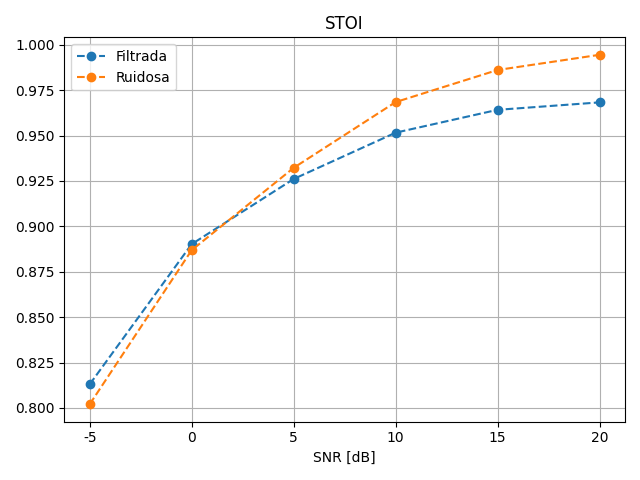
\includegraphics[scale=0.8]{images/ch7/stoi_by_snr.png}}
	\caption{STOI en función de la SNR.}
	\label{fig:ch7_stoi_by_snr}
\end{figure}

\begin{table}
	\centering
	\begin{tabular}{ |c|c|c|c|c|c|c|c| } 
		\hline
		SNR [dB] & $-5$ & $0$ & $5$ & $10$ & $15$ & $20$ & Media \\ 
		\hline
		STOI - Ruidosa & 0.67 & 0.80 & 0.89 & 0.94 & 0.98 & 0.99 & 0.88 \\
		STOI - Filtrada & 0.70 & 0.81 & 0.89 & 0.93 & 0.95 & 0.96 & 0.87 \\
		\hline
	\end{tabular}
	\caption{STOI en función de la SNR.}
	\label{table:ch7_stoi_by_snr}
\end{table}


En la figura \ref{fig:ch7_stoi_by_noise_type} podemos ver la medida STOI en función del tipo de ruido. A diferencia de la medida PESQ, la red no logró, en promedio, mejorar la inteligibilidad de las señales ruidosas. Como vimos en la figura \ref{fig:ch7_stoi_by_snr}, a bajos SNRs logra una pequeña mejora y a altos SNRs hay una degradación importante, esta combinación genera que en promedio, la red no pueda lograr mejorar la inteligibilidad para los distintos tipos de ruidos.

\begin{figure}
	\centering
	\centerline{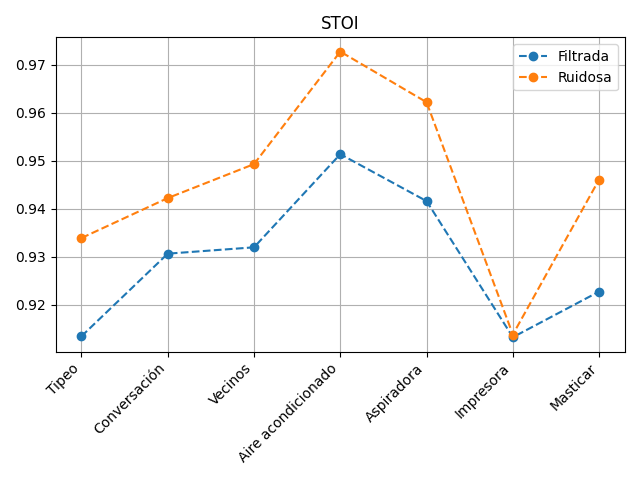
\includegraphics[scale=0.8]{images/ch7/stoi_by_noise_type.png}}
	\caption{STOI en función del tipo de ruido.}
	\label{fig:ch7_stoi_by_noise_type}
\end{figure} 


\subsubsection{Error cuadrático medio y nivel de ruido}

Al igual que para el filtro adaptativo, se obtuvo el error cuadrático medio y el nivel de ruido:

\begin{equation*}
	\text{ECM} = \frac{1}{P-1} \sum_{p=0}^{P} \frac{1}{N_p-1} \sum_{j=0}^{N_p} (\hat{s}_p(n) - s_p(n))^2
\end{equation*}

\begin{equation*}
	\text{Nivel de ruido} = \frac{1}{P-1} \sum_{p=0}^{P} \frac{1}{N_p-1} \sum_{n=0}^{N_p} (n_p(n))^2
\end{equation*}

\begin{figure}
	\centering
	\centerline{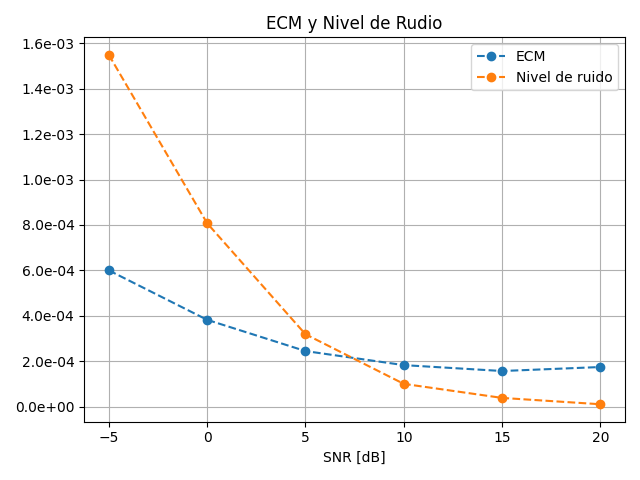
\includegraphics[scale=0.8]{images/ch7/ecm_and_noise_level.png}}
	\caption{ECM y Nivel de ruido.}
	\label{fig:ch7_mse_and_noise_level}
\end{figure}

En la figura \ref{fig:ch7_mse_and_noise_level} se muestra el error cuadrático medio y el nivel de ruido como función de la SNR. Podemos observar, que a partir de los $\SI{5}{dB}$ el error cuadrático medio se vuelve comparable con el nivel de ruido. Esto genera que la mejora media en la STOI y PESQ, a partir de los $\SI{5}{dB}$ sean cercanas a 0 o incluso negativas. En estos casos, la señal de habla filtrada tiene un nivel de ruido similar a la señal de habla ruidosa original, pero esta vez inducido por el error de generalización de la red.

\newpage

\section{Análisis comparativo}

En las secciones anteriores pudimos ver el desempeño de cada filtro por separado. Veamos ahora la comparativa utilizando las medidas PESQ y STOI. En la figura \ref{fig:ch8_pesq_comparison} podemos ver la medida PESQ - Filtrada, tanto para el filtro adaptativo como para el filtro neuronal, para los distintos niveles de ruidos utilizados.

\begin{figure}[h]
	\centering
	\centerline{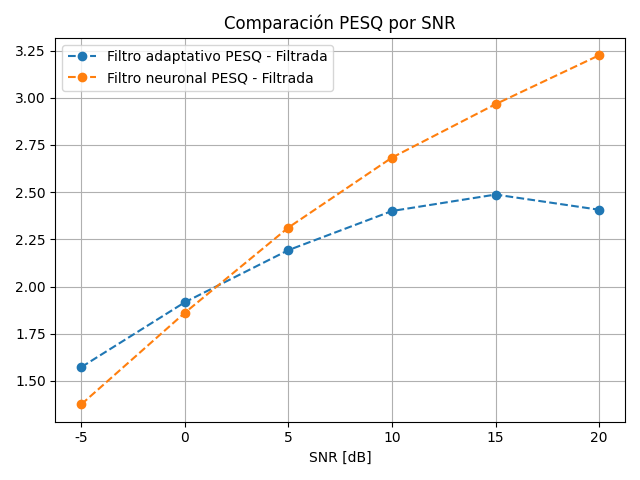
\includegraphics[scale=0.75]{images/ch8/comparison_pesq_by_snr.png}}
	\caption{Comparación PESQ en función de la SNR.}
	\label{fig:ch8_pesq_comparison_by_snr}
\end{figure}

Podemos ver en la figura \ref{fig:ch8_pesq_comparison_by_snr} que a altos niveles de ruido (SNR bajos), el desempeño del filtro adaptativo fue levemente superior, sin embargo a partir de los $\SI{5}{dB}$ el filtro neuronal superó al filtro adaptativo.	

En la figura \ref{fig:ch8_stoi_comparison_by_snr} podemos ver la medida STOI - Filtrada, tanto para el filtro adaptativo como para el filtro neuronal, para los distintos niveles de ruidos utilizados.

\begin{figure}[H]
	\centering
	\centerline{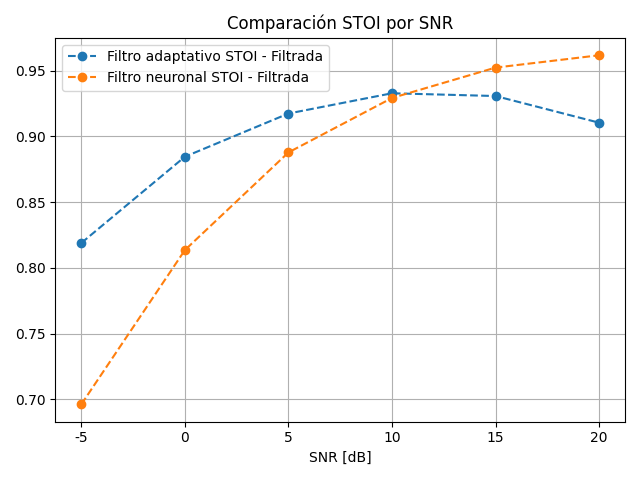
\includegraphics[scale=0.75]{images/ch8/comparison_stoi_by_snr.png}}
	\caption{Comparación STOI en función de la SNR.}
	\label{fig:ch8_stoi_comparison_by_snr}
\end{figure}

Para el caso de la STOI el filtro adaptativo fue superior en todos los casos. El filtro neuronal, a diferencia del adaptativo, trabaja en el dominio de la frecuencia lo cual lo hace mas susceptible a errores que generen una degradación en la inteligibilidad.

\newpage

\section{Conclusiones y trabajo futuro}

\subsection{Conclusiones}

El objetivo del presente trabajo fue validar la hipótesis de que un modelo de red neuronal simple, incluso utilizando la información provista por un solo micrófono, es capaz de obtener un nivel de cancelación de ruidos no-estacionarios en señales de habla, igual o mejor al obtenido con un filtro adaptativo.

A bajos niveles de SNR, el filtro neuronal, no logró el desempeño obtenido con el filtro adaptativo, pero a altos niveles de SNR, el filtro neuronal fue superior.

Dado los resultados obtenidos, lo más razonable sería utilizar el filtro adecuado para las condiciones de ruido en las que se está trabajando. En condiciones de alto nivel de ruido sería conveniente utilizar un filtro adaptativo y, en condiciones de bajo nivel de ruido, utilizar un filtro neuronal. Sin embargo, el filtro neuronal tiene la ventaja tecnológica de no necesitar dos micrófonos, por lo que sería interesante trabajar en heurísticas que permitan mejorar el desempeño del filtro neuronal en condiciones de alto nivel de ruido, de manera de lograr desempeños similares o mejores a los del filtro adaptativo.

En relación a los tipos de ruido no se observó que un filtro sea superior al otro en ciertas clases de ruido. Particularmente para el caso PESQ el filtro neuronal fue superior en todas las clases de ruido y en el caso de STOI el filtro adaptativo fue superior en casi todas las clases de ruido.

\subsection{Trabajo futuro}

El presente trabajo deja abiertos distintos aspectos a profundizar que permitirían seguir desarrollando el filtrado de ruidos en señales de habla. Veamos algunos de ellos.

Para lograr un mayor desempeño en la mejora de la inteligibilidad se debe experimentar con otras funciones de costo para el entrenamiento de la red. En lugar de utilizar el error cuadrático medio, diseñar una función de costo que se encuentre correlacionada directamente con la inteligibilidad. Con esto, lograríamos balancear la mejora en la calidad del audio con la mejora en la inteligibilidad y así obtener un resultado final superior.

En el caso de uso del filtro adaptativo, donde se cuenta con dos micrófonos, se podría aprovechar de manera más efectiva la información suministrada por ambos, incluso sin la problemática relacionada con la diafonía. Esto sería, diseñar un modelo de red neuronal que permita procesar ambas señales al mismo tiempo y utilice la información relevante de cada una para lograr generar una señal filtrada superior a la obtenida con un solo micrófono.

Por último se podría explorar el uso de la red neuronal para predecir los parámetros de un modelo de señal de habla conocido. Por ejemplo, se podría utilizar el modelo de la figura \ref{fig:ch3_voice_modeling}. La red en este caso se encargaría de estimar los parámetros del modelo, en lugar de estimar directamente la señal de habla.

\newpage

\appendix

\section{Código fuente}

Todo el código utilizado para desarrollar la presente tesis se encuentra disponible públicamente en el siguiente repositorio de código \url{https://github.com/desposito-fi-uba/tesis}

\newpage

\bibliographystyle{ieeetr}
\bibliography{refs}

\end{document}